\chapter{基于脉搏波的子痫前期识别分析软件系统的设计与实现}
\section{引言}
此前各章中均涉及了一定的软件与算法设计,在这些工作的基础上,本章介绍了一款基于PPG信号的子痫前期(PE)识别分析软件系统的设计与实现过程。在分析具体功能需求后,
选取跨平台客户端+云服务器的方案进行整体设计,以期完成以下四部分内容:PPG信号的预处理与特征计算生成;PE识别模型的本地化训练与生成;跨平台的多客户端软件设计;
云服务器端软件设计与PE识别模型的部署。对其中涉及的算法设计与软件开发进行详细的介绍,并对软件系统简单地进行了功能性的验证与测试。

本章研究内容的框架图如\autoref{fig:frameworks6}所示。

\begin{figure}[htbp]
    \centering
    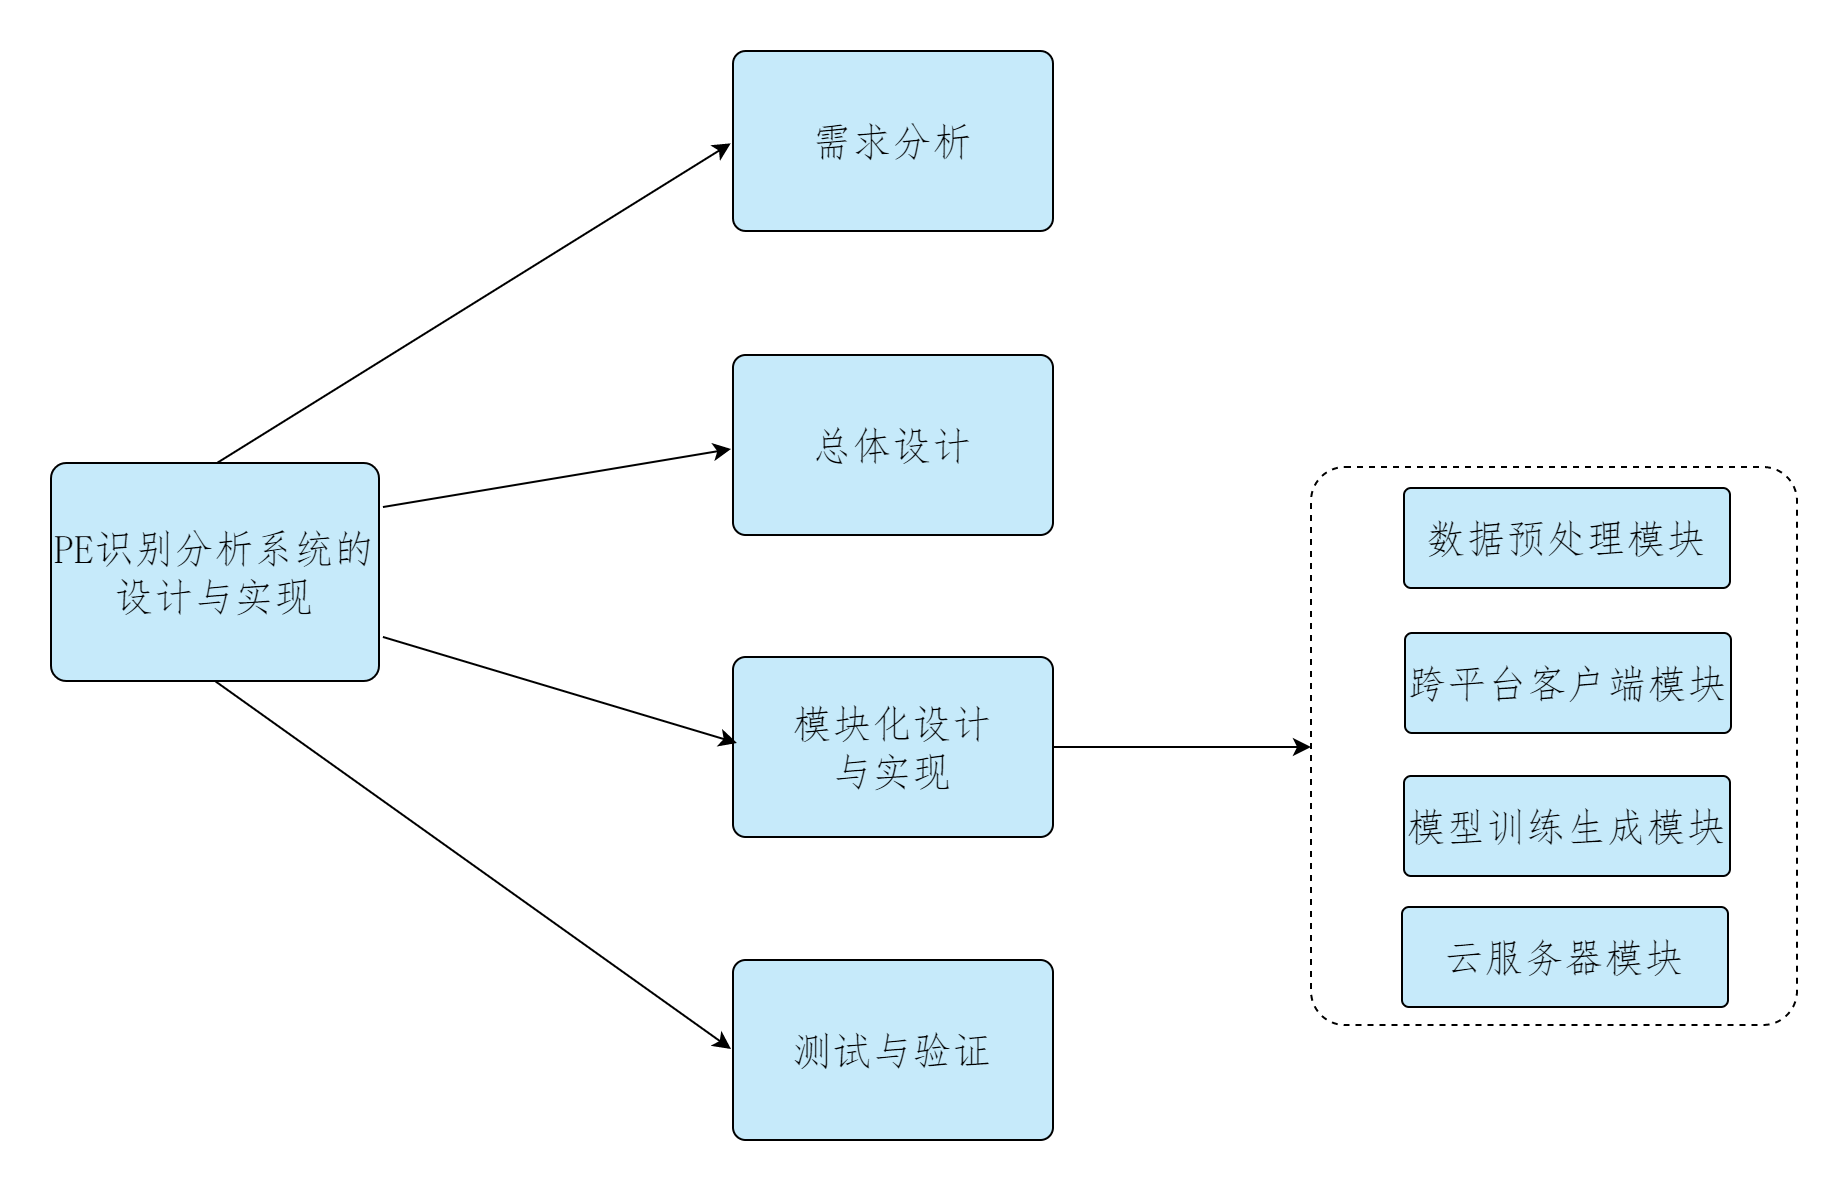
\includegraphics[width=0.9\linewidth]{software/frameworks6}
    \caption{\label{fig:frameworks6}第六章研究内容框架图}
\end{figure}

\section{需求分析}
%如本研究中绪论中所介绍的,尽管移动智能医疗与可穿戴式设备已经取得了长足的发展,但现阶段PE的微型化智能化检测技术仍处于起步阶段,国内外相关研究匮乏。
由于PE的高危害性,实现PE的早期检测识别诊断无疑可以极大地保证孕妇及婴儿的生命健康安全。因此,设计实现一款可以满足实验室研究、医院监护、社区检查、
居家监护等多应用场景的PE识别诊断软件综合系统具有重要的临床意义和广阔的市场前景。另一方面,上述软件系统在保证完整分析功能的基础上,
应支持软件自身更新迭代导致的各种变化。这要求软件系统在开发伊始就需要考虑不同的升级需求与应用情景,进行一定的兼容性设计,通过引入软件开发的
代码复用与模式设计等技术,增加软件系统的健壮性与复用性\cite{CJ2020,Enrich2018,Gamma1993}。

因此,软件系统需要满足以下具体需求:

一、完整的核心分析功能

软件系统需具备完整的PE分析功能,包括不限于对原始数据进行预处理、提取计算相关特征、构建分析数据集、对数据集进行清洗、特征提取、
识别分类模型训练和生成及最后对新数据进行预测分类等。

二、可更新迭代的处理算法

上述核心分析功能的各环节中均会涉及到一定的处理算法,如数据预处理时的滤波检波算法、特征提取时的各种新型参数的计算算法以及识别模型的机器学习训练生成算法等。
软件系统需要支持对以上算法的更新与迭代,避免由于算法的调整、切换、更新、迭代等操作引发大量的代码修改与重构等问题。

三、可动态调整的识别模型

在第五章已经介绍过,多种机器学习算法均在PE的识别分析中得到了应用。软件系统需要支持对这些由不同算法生成的不同识别模型的切换,
针对需要预测的新数据,保证返回对应模型的预测结果。

四、有效的数据管理

在上述功能需求中可以发现,除最基本的原始数据外,系统还需要对二次提取的特征参数、基础数据集划分、PE识别模型及其训练超参数等多种数据进行管理。
如何高效、有序的管理各类原始数据及中间数据也是软件系统需要解决的问题之一。

五、云服务器+跨平台客户端

考虑到软件系统在多种场景下不同的使用需求,采取云服务器与客户端结合无疑是最优的设计解决方案。由于智能便携式设备的普及,
PC端与移动端均需开发对应的客户端。

六、完备的日志记录

由于软件系统模块繁多、功能齐全,为方便开发过程中的调试、测试,同时方便部署到生产环境之后评估软件系统的运行状态,软件系统也需要具有完备的日志记录功能,
以便能够随时定位、复现、调试可能出现的问题。

七、数据源兼容性

保持对不同数据源的兼容性也是软件分析系统需要重点解决的问题之一。对于采集得到的数据,不同硬件设备使用的电子元器件、传感器等在性能参数上的区别可能导致
采集得到的数据在信号质量、采样率、分辨率及数据存储与解析格式等方面均存在差异;而由数据库得到的数据,其字段信息也极容易出现差异。

八、其他拓展性

在本研究中,PPG信号是目前使用的唯一人体电生理信号。但随着高性能的多通道多参数生理信号(如ECG、BCG、EEG)数据采集设备的普及,这些信号
也存在着联合分析的可能\cite{Chen2020,Kachuee2015,LMX2017}。此外,尽管软件分析系统是为PE的识别分析为初衷进行设计,其核心分析功能可作为类似研究的参考模板,
软件分析系统在进行设计时也可以考虑整体的移植性。

\section{总体设计}

为实现上小节中具体的开发需求,软件分析系统按照低耦合、高拓展的原则进行了模块化、功能化的设计。其中,
每一模块只处理某一类特定任务,在实现模块功能高内聚性的同时保持模块间的松耦合性。

一、模块化设计

软件系统的核心分析功能被拆分为四个独立的功能模块分别实现,整体设计框图如\autoref{fig:scas}所示。
\begin{figure}[htbp]
    \centering
    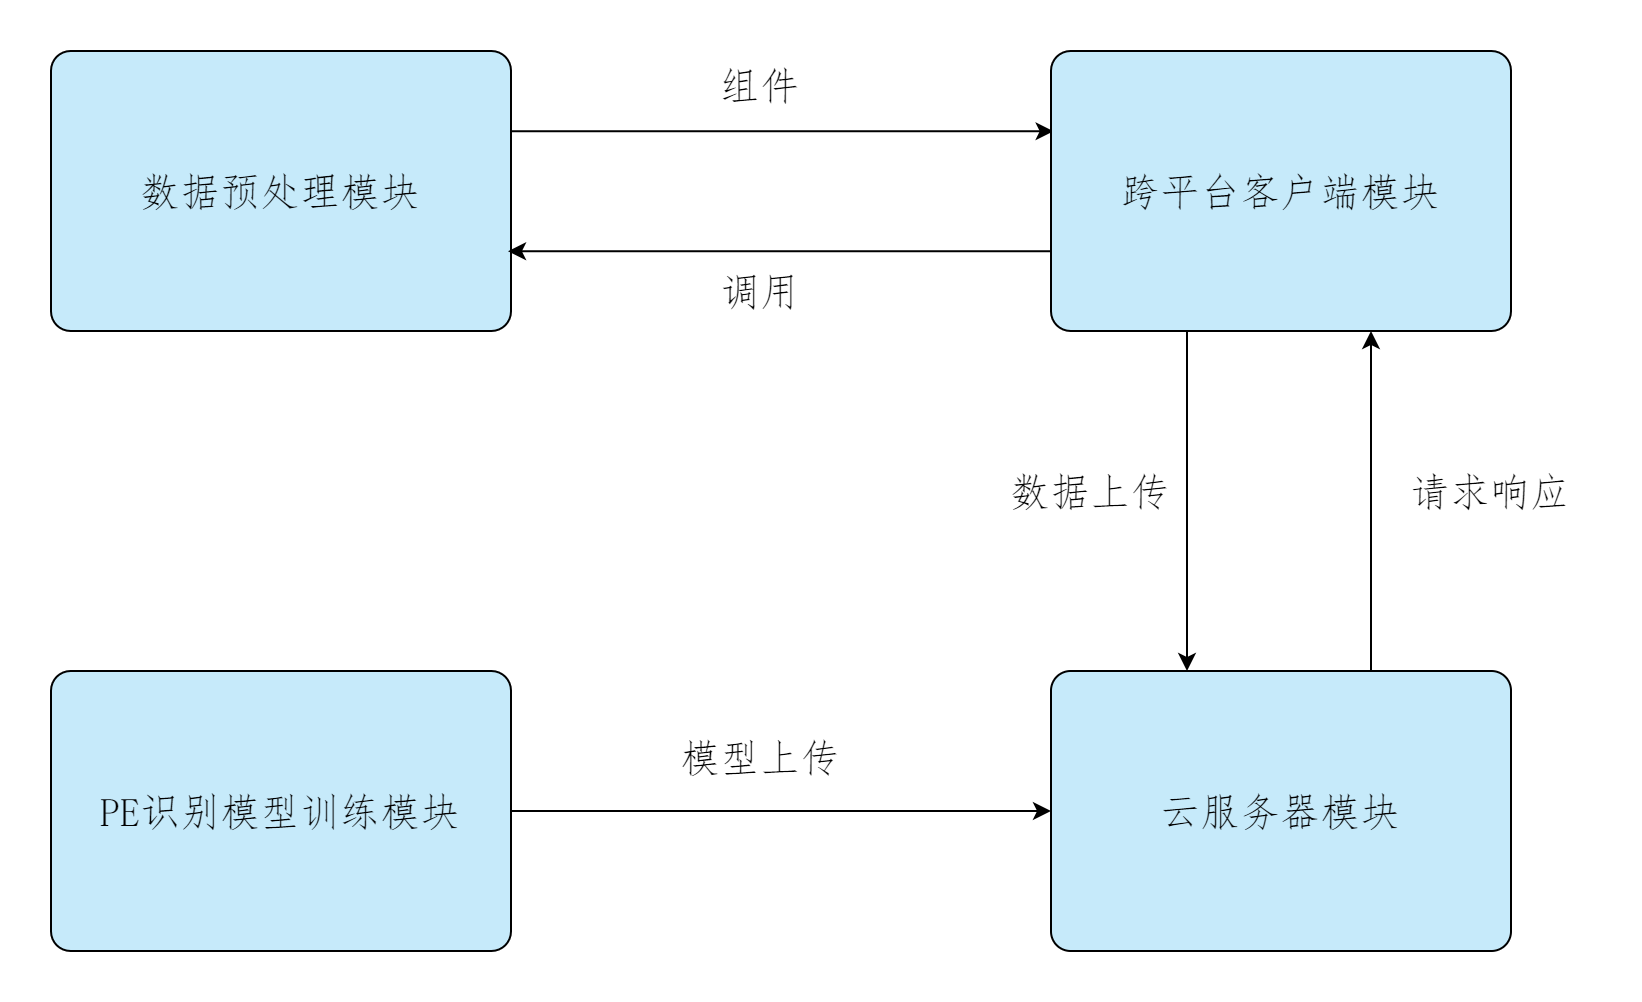
\includegraphics[width=.65\linewidth]{software/scas}
    \caption{\label{fig:scas}软件分析系统的多模块设计框架图}
\end{figure}

1、数据预处理模块

数据预处理模块主要负责从原始PPG信号中提取数据特征,包括数据的读取、PPG信号的滤波降噪、波形的检测识别、特征定义及计算等具体处理任务。
为满足跨平台使用需求,本模块涉及的处理算法或处理步骤需具有平台独立性,不依赖的操作系统或生产运行环境。

2、跨平台客户端模块

为满足多种可能的应用场景,软件系统需要完成跨平台客户端开发。上述数据预处理模块可在跨平台客户端模块中得到调用,PPG波形的特征数据经客户端
经由互联网被发送至云服务器端进行处理分析,云服务器的处理分析结果也会经由互联网发送返回给客户端进行展示。

3、PE识别模型训练生成模块

在获取客户端传输的数据后,PE识别模型训练生成模块需要负责原始数据特征的整理与数据集划分。
在此基础上,完成PE识别模型的训练生成与评估、识别模型的超参数优化等工作。此外,识别模型本身及其训练所需的超参数也需被保存并上传至云服务端,方便后续新数据进行预测分析。

4、云服务器模块

云服务器模块负责管理由客户端发送来的数据信息、管理系统具体PE识别模型。当客户端发来新的数据并请求分析时,云服务器模块从客户端发送来的参数信息中确定具体使用的识别模型,
将数据交由对应的模型进行分析后,将分析结果返回至发出请求的具体客户端。

二、设计原则的应用

为使上述多功能、多模块化软件系统的开发能顺利进行,必须遵循计算机软件开发领域一定的设计思想与开发原则。

1、面向对象编程

面对对象编程(object oriented programming,OOP)是一种普及的计算机编程架构,通过尽可能模拟人类的思维方式,OOP使得软件的开发方法与过程尽可能接近人类认识世界、
解决现实问题的方法和过程。OOP可以简化复杂的编程过程,使软件开发的逻辑更为简单。

2、设计模式

设计模式(design pattern,DP)是计算机软件设计中对某些特定问题的优化解决方案的总结\cite{Gamma1993,Enrich2018}。
在程序开发过程中使用设计模式,可提高代码可读性并方便重用代码,在一定程度上避免了代码重构。

三、编程语言与开发环境

软件系统各模块所使用的编程语言与开发环境工具如\autoref{tab:ides}所示。各模块所使用的一些重要组件或开源库也在表格中进行了说明,这些组件的具体介绍可参见后续内容。

\begin{longtblr}
    [
        theme                   = {zju},
        caption                 = {不同模块使用的编程语言与开发环境},
        label                   = {tab:ides},
    ]
    {
        width                   = \linewidth,
        colspec                 = {X[0.5,c,m]X[1.5,c,m]X[1,c,m]X[1,c,m]X[2.8,c,m]X[1.5,c,m]X[1.5,c,m]},
        hline{1,Z}              = {\thickline},
        hline{2}                = {\thinline},
        rowhead                 = 1,
        row{1}                  = {font=\headfont},
        row{2-Z}                = {font=\nonheadfont},
        cell{3}{1-2}            = {r=2,c=1}{c,m},
        cell{2}{4}              = {r=3,c=1}{c,m},
        cell{2}{5-6}            = {r=2,c=1}{c,m},
        cell{5}{3-6}            = {r=2,c=1}{c,m},
    }
    序号 & 模块 & 平台 & 开发语言 & 版本 & 开发工具 & 其他组件或库 \\
    1 & 数据预处理 & / & Java & OpenJDK(16.0.2)\cite{openjdk} & VS Code & fastjson\cite{fastjson} \\
    2 & 客户端 & PC & Java & OpenJDK(16.0.2) \cite{openjdk}& VS Code & httpClient\cite{httpClient}、JFreeChart\cite{JFreeChart}、log4j\cite{log4j} \\
    2 & 客户端 & Android\cite{android} & Java & Android Studio default JDK(11.0.12)  & Andoird Studio & retrofit\cite{retrofit}、MPAndroidChart\cite{MPAndroidChart} \\
    3 & 模型训练 & / & Python & 3.9.7 & PyCharm & Sklearn\cite{scikit-learn}、logging\cite{logging} \\
    4 & 云服务器 & / & Python & 3.9.7 & PyCharm & Sklearn\cite{scikit-learn}、Django\cite{django}、logging\cite{logging} \\
    
\end{longtblr}

\section{模块设计与实现}

针对此前提出的多项具体需求,本小节将详细介绍总体设计中确定的四个模块的设计与开发过程。
\subsection{数据预处理模块}

数据预处理模块整体的处理流程如\autoref{fig:preprocess2}所示。下面依次介绍\autoref{fig:preprocess2}中各步骤的详细设计。
\begin{figure}[htbp]
    \centering
    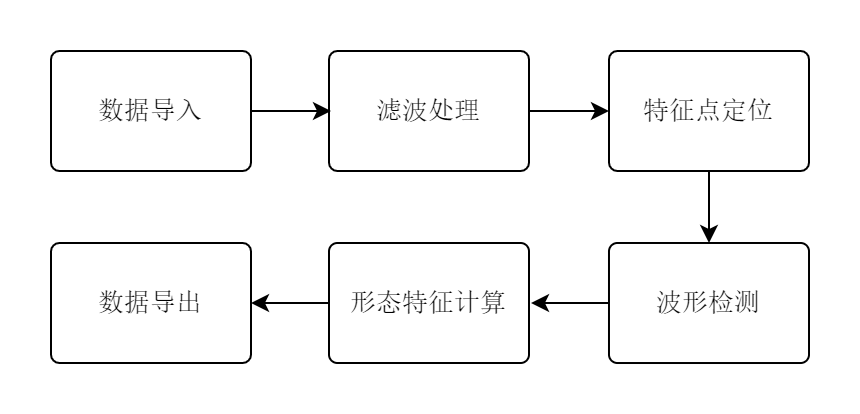
\includegraphics[width=.6\linewidth]{software/preprocess}
    \caption{\label{fig:preprocess2}数据预处理模块流程图}
\end{figure}
\begin{figure}[htbp]
    \centering
    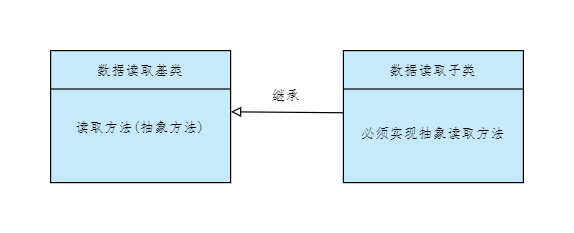
\includegraphics[width=.55\linewidth]{software/read}
    \caption{\label{fig:template}数据导入设计示意图}
\end{figure}
一、数据导入

为兼容读取由不同硬件设备采集得到的原始数据,软件系统将数据读取过程进行了抽象,如\autoref{fig:template}所示。
当需要读取具体来源或特定格式的数据时,必须重新定义实现抽象基类的一个子类,并在子类中详细实现具体的读取方法。


该机制延迟实现了读取的具体处理过程,隔离了硬件差异、数据格式等原因对系统其他功能的影响,也保证了系统整体的灵活性。
在这种设计下,目前软件系统支持的硬件设备包括GE B650、迈瑞ePM 15M生理信号监护仪等多种医用监护仪,
同时也支持研究团队自研的多生理参数采集设备。

二、滤波处理

生理信号的滤波过程一般会涉及多种类型的数字滤波器甄选与参数调整,性能最佳的滤波器往往需要对多种滤波器调参后综合测评后才能判别得到。
为使软件分析系统能在多种滤波器之间灵活切换,使用了DP中的模板方法(Template Method)对这一过程进行了设计\cite{Enrich2018},如\autoref{fig:template2}所示。
\begin{figure}[htbp]
    \centering
    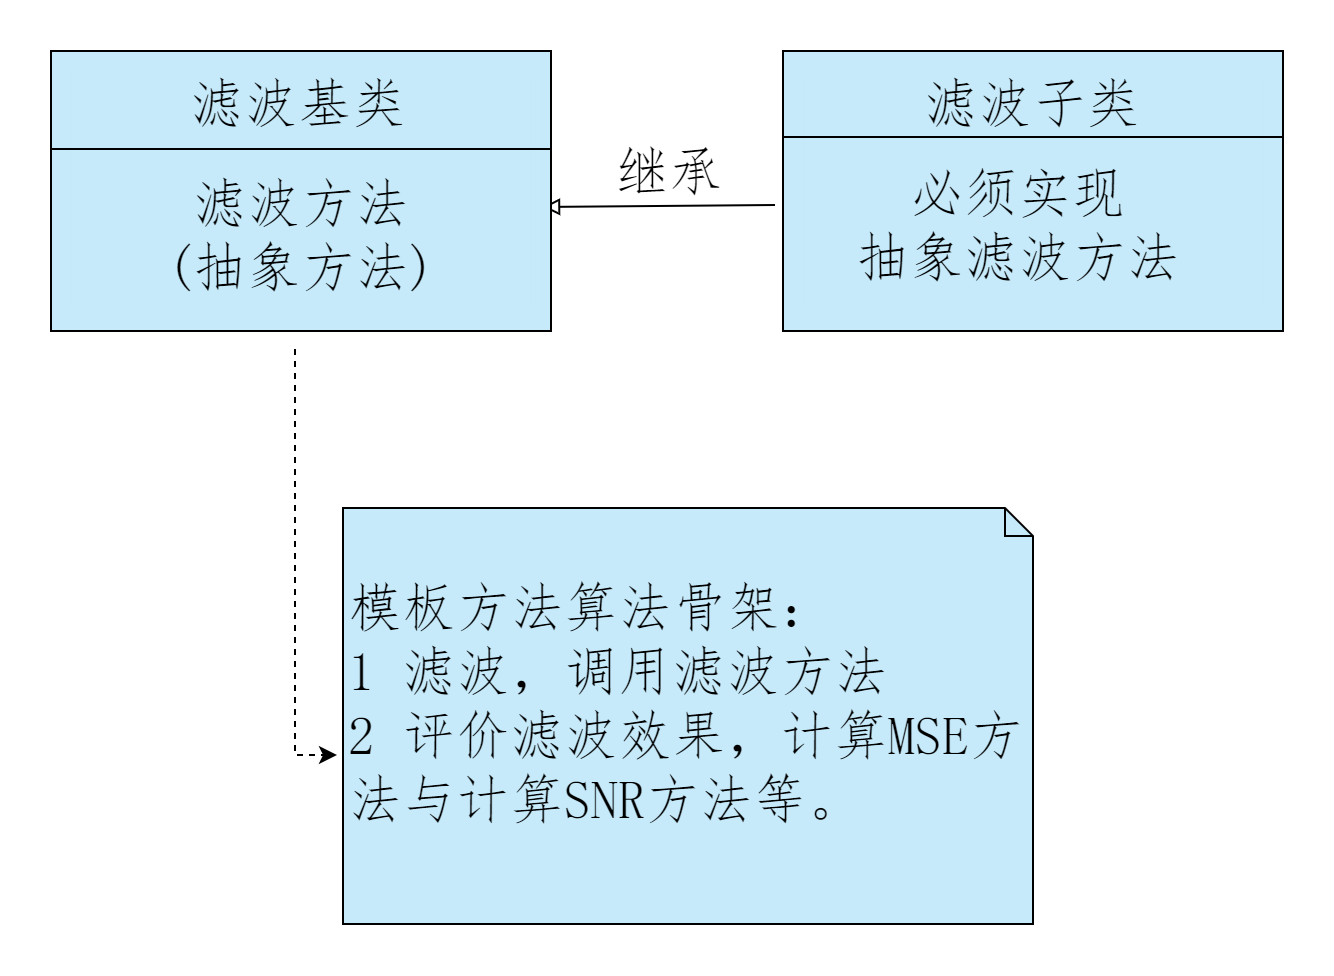
\includegraphics[width=.5\linewidth]{software/template}
    \caption{\label{fig:template2}滤波处理设计示意图}
\end{figure}


与\autoref{fig:template}不同的是,在\autoref{fig:template2}中,滤波过程所对应的抽象基类中除定义了模板方法外,还定义了其他评价滤波效果的相关方法。
常用于评价滤波效果的均方误差与信噪比等指标可以设计为滤波基类的业务方法;而带通滤波器、小波滤波器等多种经典滤波算法可以在不同的滤波子类滤波方法中实现。

三、特征点定位与波形检测

本研究对PPG波形的检测过程进行了模式设计,
结合模板方法与工厂方法(Factory Method)\cite{Enrich2018},提出了一种基于初筛—复核—决策(screening-checking-deciding,SCD)的新型算法。
SCD算法的处理流程如\autoref{fig:detect2}所示,其详细介绍可参见论文第三章。
% 由于特征点定位与波形检测的详细算法过程已经在第三章中详细介绍过,此处对其算法原理不再赘述。
\begin{figure}[htbp]
    \centering
    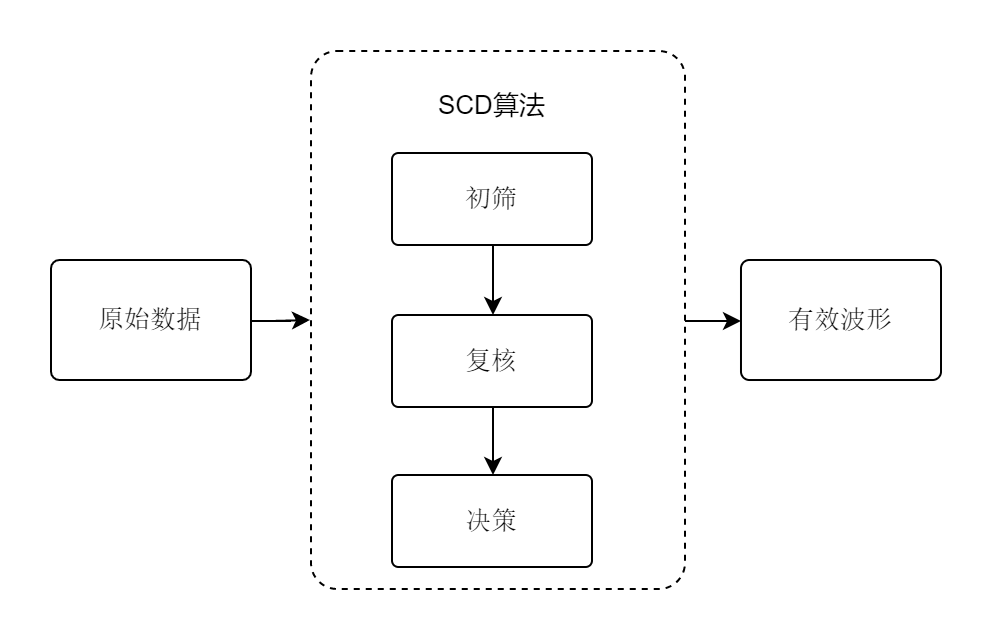
\includegraphics[width=0.7\linewidth]{software/scd}
    \caption{\label{fig:detect2}SCD算法检测流程示意图}
\end{figure}

四、特征计算

针对本论文第四章中定义的大量PPG形态学的特征参数的计算,软件系统使用单例程模式(Singlon)该过程进行了模式设计\cite{Enrich2018},
如\autoref{fig:singleton}所示。

\begin{figure}[htbp]
    \centering
    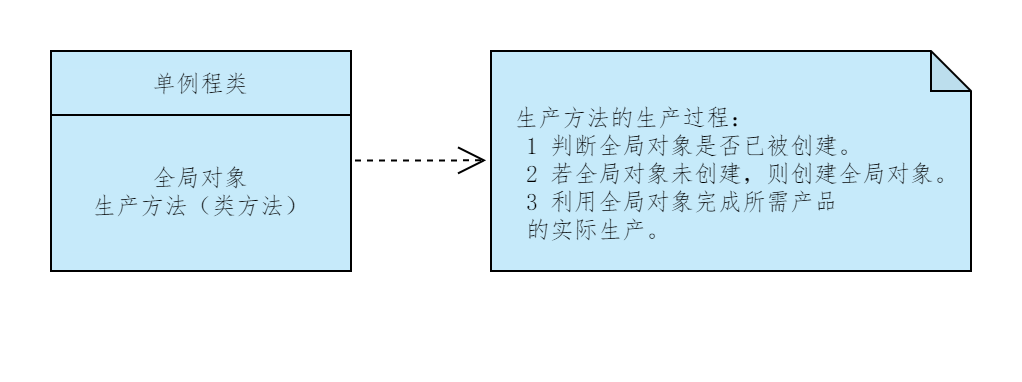
\includegraphics[width=.9\linewidth]{software/singleton}
    \caption{\label{fig:singleton}单例程模式原理示意图}
\end{figure}

单例程模式的原则是保证一个类仅有一个实例,并提供该实例的唯一全局访问点。
由于PPG时域特征种类繁多,本研究在时域特征的抽象基类中定义了模板方法,
由该模板负责调用特征的计算方法。
在初次被调用时,生产方法会创建并保存单例程类本身的一个全局对象,并由全局对象完成生产返回所需产品;
此后的调用直接均由全局对象完成生产。单例程模式可以提升软件系统的工作效率、降低内存资源的消耗。

另外,计算某些特定的特征可能需要一定的先导条件,即预先计算某些先导特征。因此,预处理模块在时域特征的抽象基类额外定了两个属性$Order$与$Prefixes$,
其中$Order$存储了当前特征的计算顺序,$Prefixes$存储了其先导特征的顺序。
按照先导条件从无到有、从少到多、从简单到复杂的原则,在初始化特征时,给每个具体实现子类设置好其计算顺序与先导依赖,
随后按照所有特征的$Order$遍历计算,即可保证所有特征的计算依赖都被满足。

五、数据导出

当PPG信号的预处理分析完成后,由于采取了OOP设计,此时内存中的PPG特征是以PPG波形为单位存在的。而在本研究中,多种新设计的特征参数往往是以向量的形式出现,
因此,内存中的PPG特征数据实际存在着波形——特征——向量(pulse-feature-vector)的二级树状结构。
% 此外信号特征算法出现引入了新的信号特征、对已有特征值数值的保存形式进行更改等更迭将会直接引起数据存储格式的变化。
常见的基于列表式的CSV、TXT等格式对这种树状数据格式的支持较差,因此,软件分析系统选用了JavaScript对象标记法(JavaScript object notation,JSON)\cite{json}
作为数据交换格式,并利用了中国阿里巴巴公司的开源JSON解析库fastjson\cite{fastjson}进行相关功能开发。
JSON格式对数组类数据有着更好的支持,有着更快的读写速度与更高的存储效率。


六、多生理参数的兼容接口

为保留后续研究引入更多人体电生理信号进行分析的可能,
软件系统进一步设计了表征一般生理信号的抽象基类$AbstractBMESignal.class$。
PPG信号作为上述抽象生理信号的具体子类被设计为$Pulse.class$,而上文中介绍的具体处理过程均是对抽象基类$AbstractBMESignal.class$中各抽象方法的具体实现。
后续若有其他生理信号的分析需求,可以视情况
拓展实现心电$ECG.class$、脑电$EEG.class$等。由于这些子类都继承自$AbstractBMESignal.class$,因此可以确保这些子类具有相同的函数接口,方便兼容拓展。

\subsection{跨平台客户端模块}

在数据与处理模块的基础上,软件系统利用Java编程语言分别完成了PC客户端与Android客户端的设计开发,以下为具体介绍。

一、预期用户与使用场景

为满足需求分析中所期的实验室研究、医院监护、社区检查及居家监护等多种不同的使用场景,软件系统基于Java语言完成了跨平台客户端设计与研发以满足
科研人员、临床医生及普通用户等不同身份的使用者的不同使用需求。其中,PC端的主要使用用户为实验室分析研究人员与临床医生;
后者的使用人群包括不限于临床医生、社区工作人员及普通居家人群。

跨平台客户端核心功能相同,但不同平台下的功能也略有区别:PC客户端的软件功能更精细,还提供了
包括为实验室研究人员设计的更精细化的、可提高SCD算法检波效果的人工波形校验功能、提供了一定意义上的多段数据的自动化分析功能与详细的操作日志记录等功能;
而Android客户端则更加聚焦移动端操作的便携性与使用流程的简化,更聚焦于软件核心功能的操作与处理结果的展示。

二、PC客户端

软件系统借助VS Code在Windows系统下完成了PC客户端的开发。而由于Java本身的跨平台特性\cite{openjdk},该客户端也可方便在Linux等其他系统下进行编译运行。

1、功能与界面

PC客户端的交互界面如\autoref{fig:pc_ui}所示。%\autoref{tab:pc_ui}对\autoref{fig:pc_ui}中软件界面的相关功能进行了进一步的说明。
其中,文件菜单包含了选择需要打开的原始数据与经分析后特征数据的上传;编辑菜单可以完成数据的预处理、分析等功能;
批处理菜单提供了大量数据进行处理分析的便捷操作方式;而帮助菜单则给出软件开发单位、软件版本号等信息。这些功能的进一步说明可参考\autoref{tab:pc_ui_menu}。
% 软件交互界面的波形显示区域可以展示当前打开数据文件的波形图,支持通过鼠标完成拖动、缩放等功能;对波形的波峰波谷等特征点的分析也在\autoref{fig:pc_ui}中有所标示。
% 与此同时,PC端软件也提供了较为丰富的右键菜单功能,提供了修改绘图颜色字体属性,支持选中当前波形直接复制至文件及连接打印机打印等功能。

% \begin{longtblr}
%     [
%         theme                   = {zju},
%         caption                 = {PC端软件界面功能说明},
%         label                   = {tab:pc_ui},
%     ]
%     {
%         width                   = \linewidth,
%         colspec                 = {X[1,c,m]X[3,c,m]X[1,c,m]X[3,c,m]},
%         hline{1,Z}              = {\thickline},
%         hline{2}                = {\thinline},
%         rowhead                 = 1,
%         row{odd}                = {bg=\oddcolor}, 
%         row{even}               = {bg=\evencolor},
%         row{1}                  = {font=\headfont,bg=\headcolor},
%         row{2-Z}                = {font=\nonheadfont},
%     }
%     编号 & 功能 & 编号 & 功能 \\
%     1 & 菜单栏 & 5 & 波形起点标记 \\
%     2 & 文件路径及PE状态说明 & 6 & 波形终点标记 \\
%     3 & 波形显示区域 & 7 & 右键功能菜单 \\
%     4 & 波形峰值标记 & 8 & 图例 \\
% \end{longtblr}

\begin{longtblr}
    [
        theme                   = {zju},
        caption                 = {PC端软件主菜单功能},
        label                   = {tab:pc_ui_menu},
    ]
    {
        width                   = \linewidth,
        colspec                 = {X[1,c,m]X[1.5,c,m]X[4,c,m]},
        hline{1,Z}              = {\thickline},
        hline{2}                = {\thinline},
        rowhead                 = 1,
        row{1}                  = {font=\headfont},
        row{2-Z}                = {font=\nonheadfont},
        cell{2}{1}              = {r=3,c=1}{c,m},
        cell{5}{1}              = {r=2,c=1}{c,m},
        cell{7}{1}              = {r=4,c=1}{c,m},
        cell{11}{1}             = {r=3,c=1}{c,m},
        cell{14}{1}             = {r=2,c=1}{c,m},
    }
    菜单 & 子菜单 & 功能说明 \\
    文件 & 打开 & 选择需要分析的PPG文件 \\
        & 上传单个文件 & 上传单个PPG文件的处理结果至云服务器\\
    文件 & 上传目录下文件 & 上传目录下多个PPG文件的处理值云服务器端\\
    编辑 & 设置PE状态 & 标记当前PPG文件对应的孕妇的PE状态 \\
        & 波形校验 & 开启SCD算法自动校验波形 \\
        & 波形人工校验 & 启动人工校验波形功能\\
        & 导出检波结果 & 将检测到的PPG波形数据以JSON形式保存至硬盘\\
    编辑 & 特征分析 & 开始计算检测PPG波形的特征参数 \\
    编辑 & 导出并上传 & 导出当前分析的所有分析结果,并将结果上传至云服务器 \\
    批处理 & 操作说明 & 显示批处理操作的帮助文档\\
        & 生成模板 & 选择要批处理分析的文件夹路径,并在目录下生成批处理模板\\
        & 开始批处理 & 选择经过人工调整确认过的批处理模版,开始批处理\\
    帮助 & 更新日志 & 显示软件的更新日志信息\\
        & 关于 & 显示软件的开发团队、版本信息等 \\
\end{longtblr}
\begin{figure}[h]
    \centering
    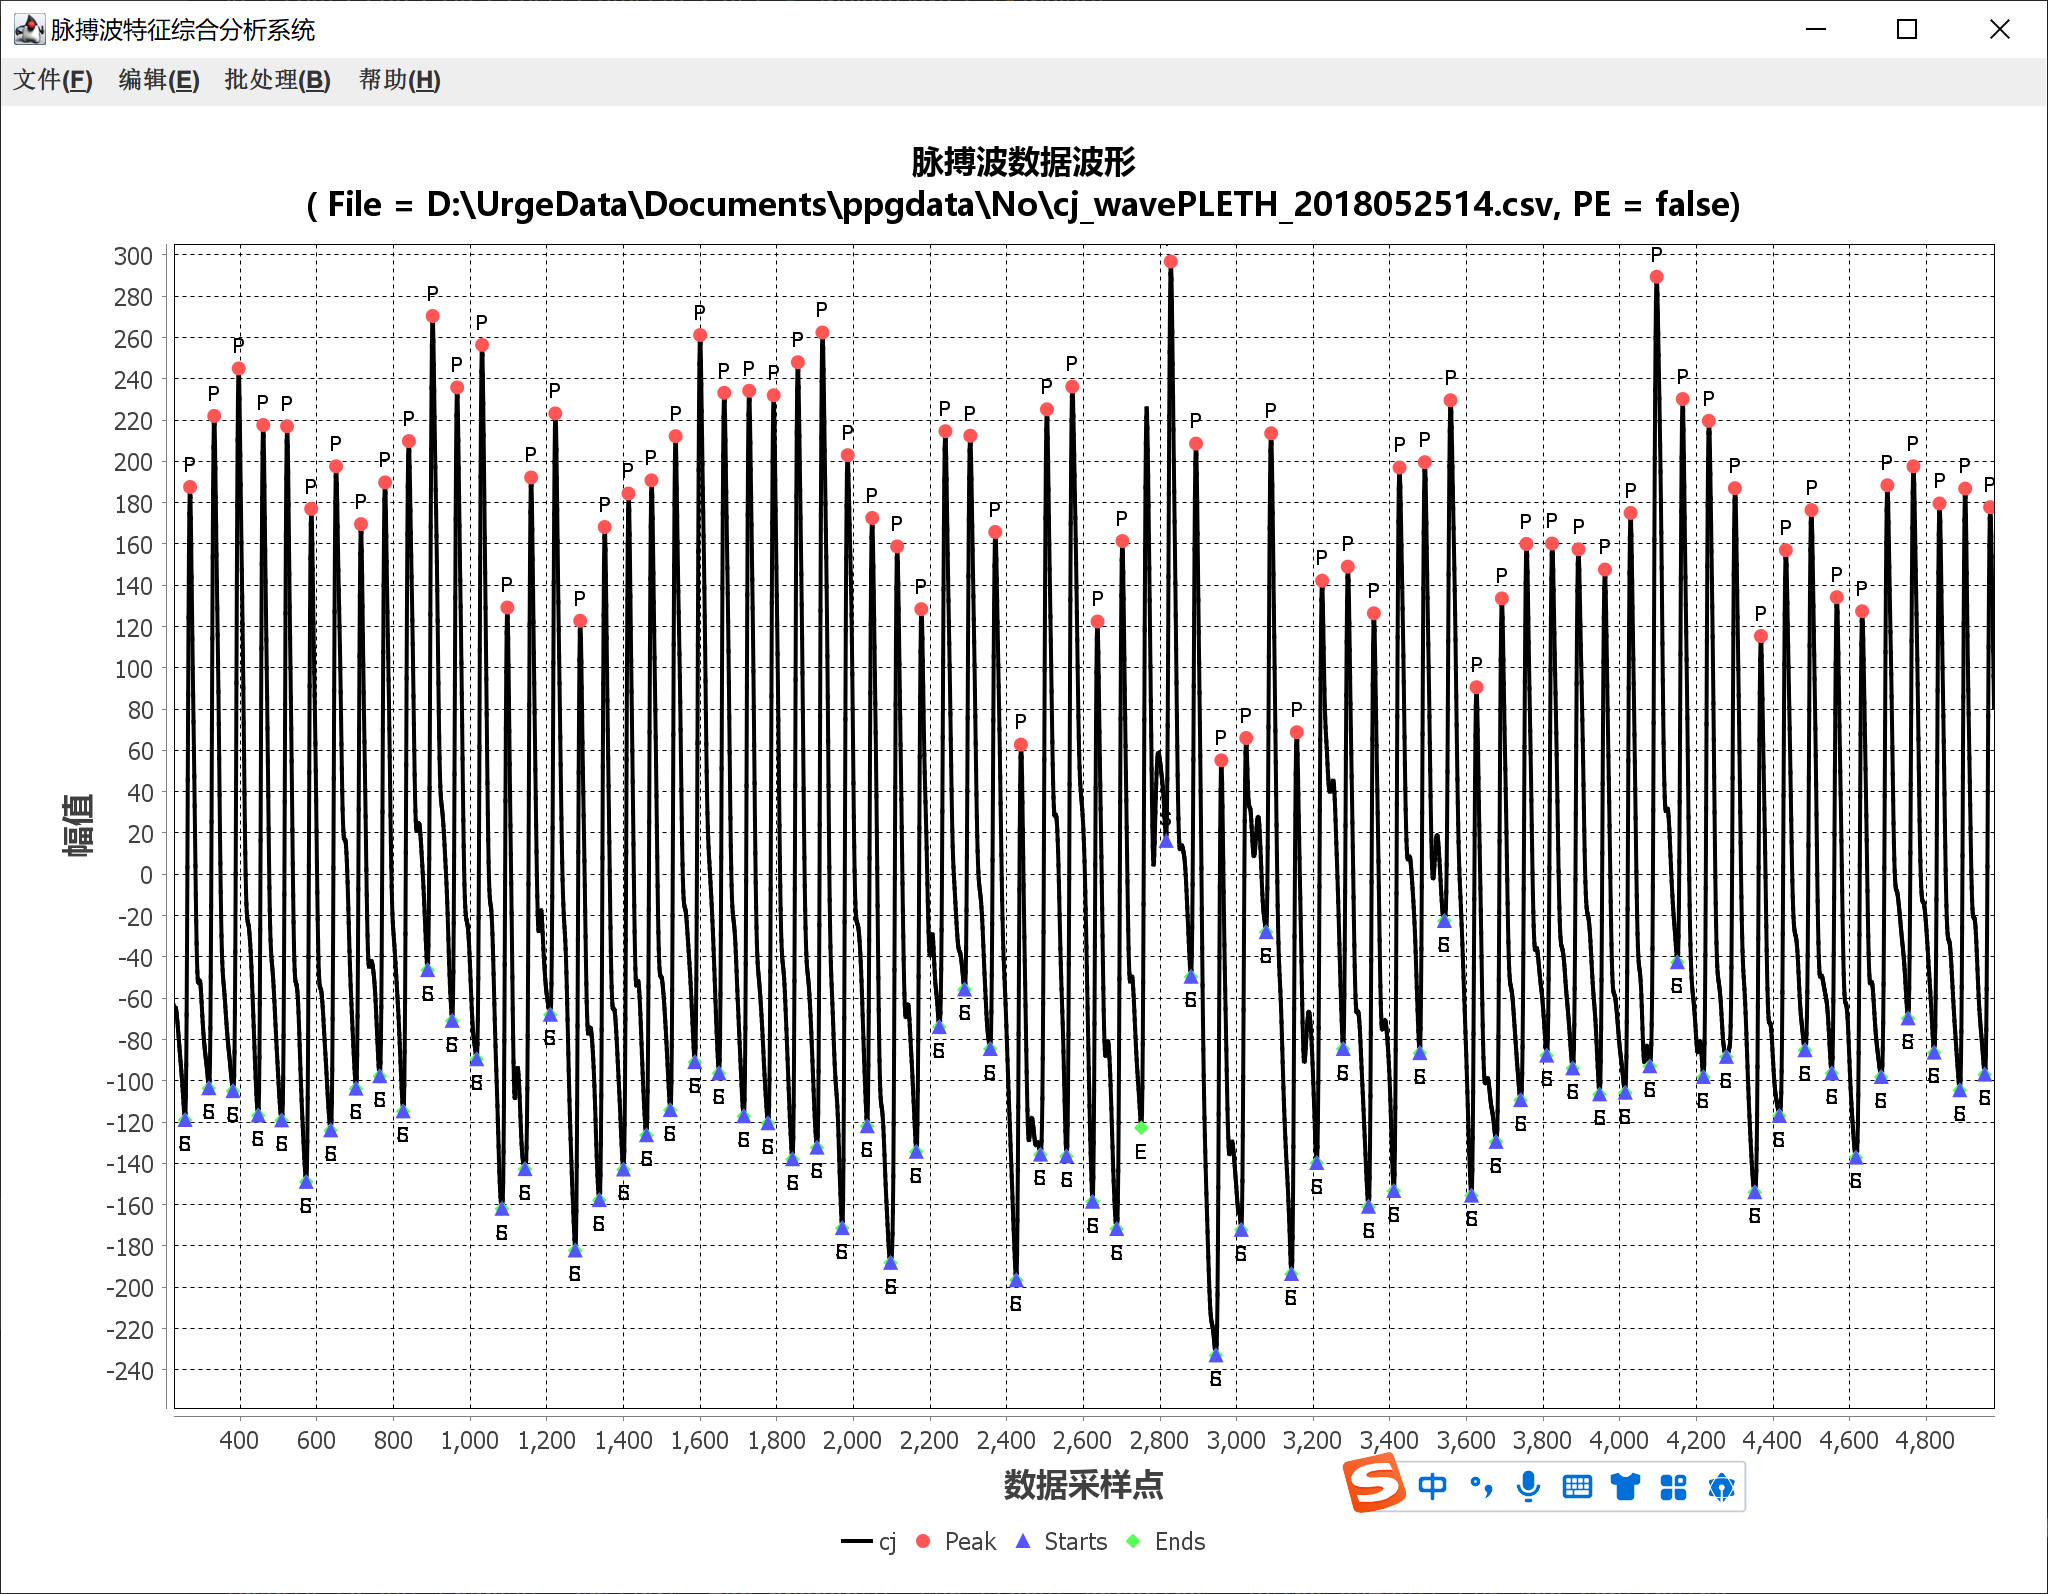
\includegraphics[width=0.9\linewidth]{software/pc}
    \caption{\label{fig:pc_ui}PC端软件界面示意图}
\end{figure}

2、处理流程与逻辑

\begin{figure}[htbp]
    \centering
    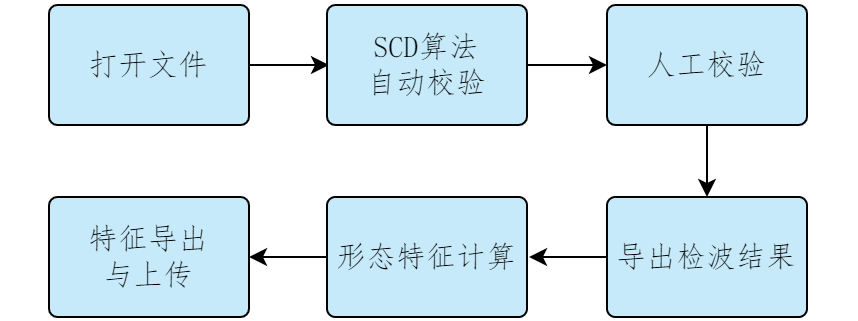
\includegraphics[width=.6\linewidth]{software/pc_process}
    \caption{\label{fig:pc_process}PC客户端程序的操作流程图}
\end{figure}

PC客户端软件正常的处理流程如\autoref{fig:pc_process}所示。在选中需要分析的PPG文件后,软件系统会自动调用SCD算法的进行波形初筛,并将筛选结果在波形显示区域进行标注。
此时,点击波形检验菜单,SCD算法的检查与投票功能会被调用,会对此前的检验结果进行调整修正。用户可以通过鼠标放大观察整段数据的检测结果,若对
检测结果有异议,可以点击波形人工校验菜单进行校正。随后,用户可以选择导出波形的检测结果,将完整波形对应的数据段以及其相对原始数据的位置等信息导出。
最后,点击特征分析可以计算PPG波形的时域特征,点击导出并上传会将波形检测结果与特征计算结果以JSON形式保存,同时上传这些数据至云服务器进行后续分析。

3、特色功能说明

1)完善的日志记录

PC客户端软件借助Apache公司的log4j(log for Java)开源项目\cite{log4j}进行软件日志管理与输出,可将软件运行过程中的运行状态和中间变量等关键信息按级别
输出到不同日志文件中,方便系统开发与调试维护。

2)人工校验波形

为解决SCD波形检测算法对某些极端数据的漏检、误检等问题,进一步提高算法的检测能力,PC客户端还额外开发了对PPG波形的人工校验功能以精细控制PPG波形的增删,如\autoref{fig:manal_check}所示。

在\autoref{fig:manal_check}中,点击其中表格当前行末的跳转至按钮,软件界面会自动放大波形并跳转至当前选择波形,方便观察细节。
当需要删除已检波形时,只需在\autoref{fig:manal_check}中取消勾选波形行末的确认按钮;当需要调整波形起点、波峰及波谷时,只需双击相应数字单元格,
输入新的采样点序号近似值;当需要新增波形时,只需点击\autoref{fig:manal_check}中的增加新波形,并输入新的波形
的起点、波峰及波谷的近似采样点序号。点击校验当前行,PC软件会自动检查当前波形,并在起点、波峰及波谷的采样点序号的邻域内自动选择更为精确的数值,并将相应操作更新至
软件的波形显示区域;而点击校验所有行则会对所有波形进行相应的处理。
\begin{figure}[htbp]
    \centering
    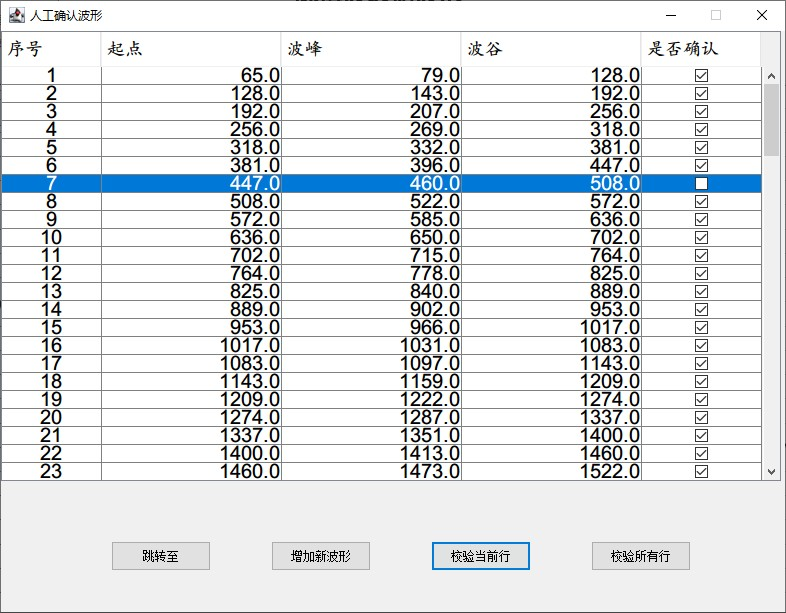
\includegraphics[width=0.8\linewidth]{software/manal_check}
    \caption{\label{fig:manal_check}PC客户端人工校验波形操作界面图}
\end{figure}

3)批处理

当PPG波形的特征算法得到更新、云服务器端的识别模型得到更新之后,可能需要对已进行过分析的PPG数据重新分析。
此时按\autoref{fig:pc_process}中的处理逻辑与流程,人工手动处理原始PPG数据无疑显得耗时、低效且繁琐,尤其是需要重新分析处理的数据量较大时。
PC客户端软件的批处理功能就是为简化上述繁琐耗时的操作流程而设计。

批量处理的核心思路是预先将多条PPG数据的处理过程中的各项具体的操作写入配置文件中,随后按照该配置文件依次处理所有PPG数据原始记录文件。
具体操作时,需选择\autoref{fig:pc_ui}中的批处理菜单,再从如\autoref{tab:pc_ui_menu}所示的子菜单中选中生成模板。生成模板操作会要求选择一个
文件夹作为批处理的根目录,该根目录下所有的有效PPG原始文件会被记录,并在根目录下生成一个空白的配置文件模板。此时,需要用户
根据实际需要,自定义每一个PPG数据文件的个性化的处理流程,包括波形的计算与调整等。当批处理配置文件由用户更新完成后,最后可点击
从\autoref{tab:pc_ui_menu}所示的子菜单中选中开始批处理,选择打开该配置文件,等待PC客户端处理完成即可。

三、Android客户端

软件系统借助Android Studio在Windows系统下完成了Android客户端的开发,并在中国小米公司生产的Redmi Pad SE上测试通过。
其中,Redmi Pad SE的Linux内核版本为5.10.101,Android版本为12。
\begin{figure}[htbp]
    \centering
    \subfigure[默认界面]{
    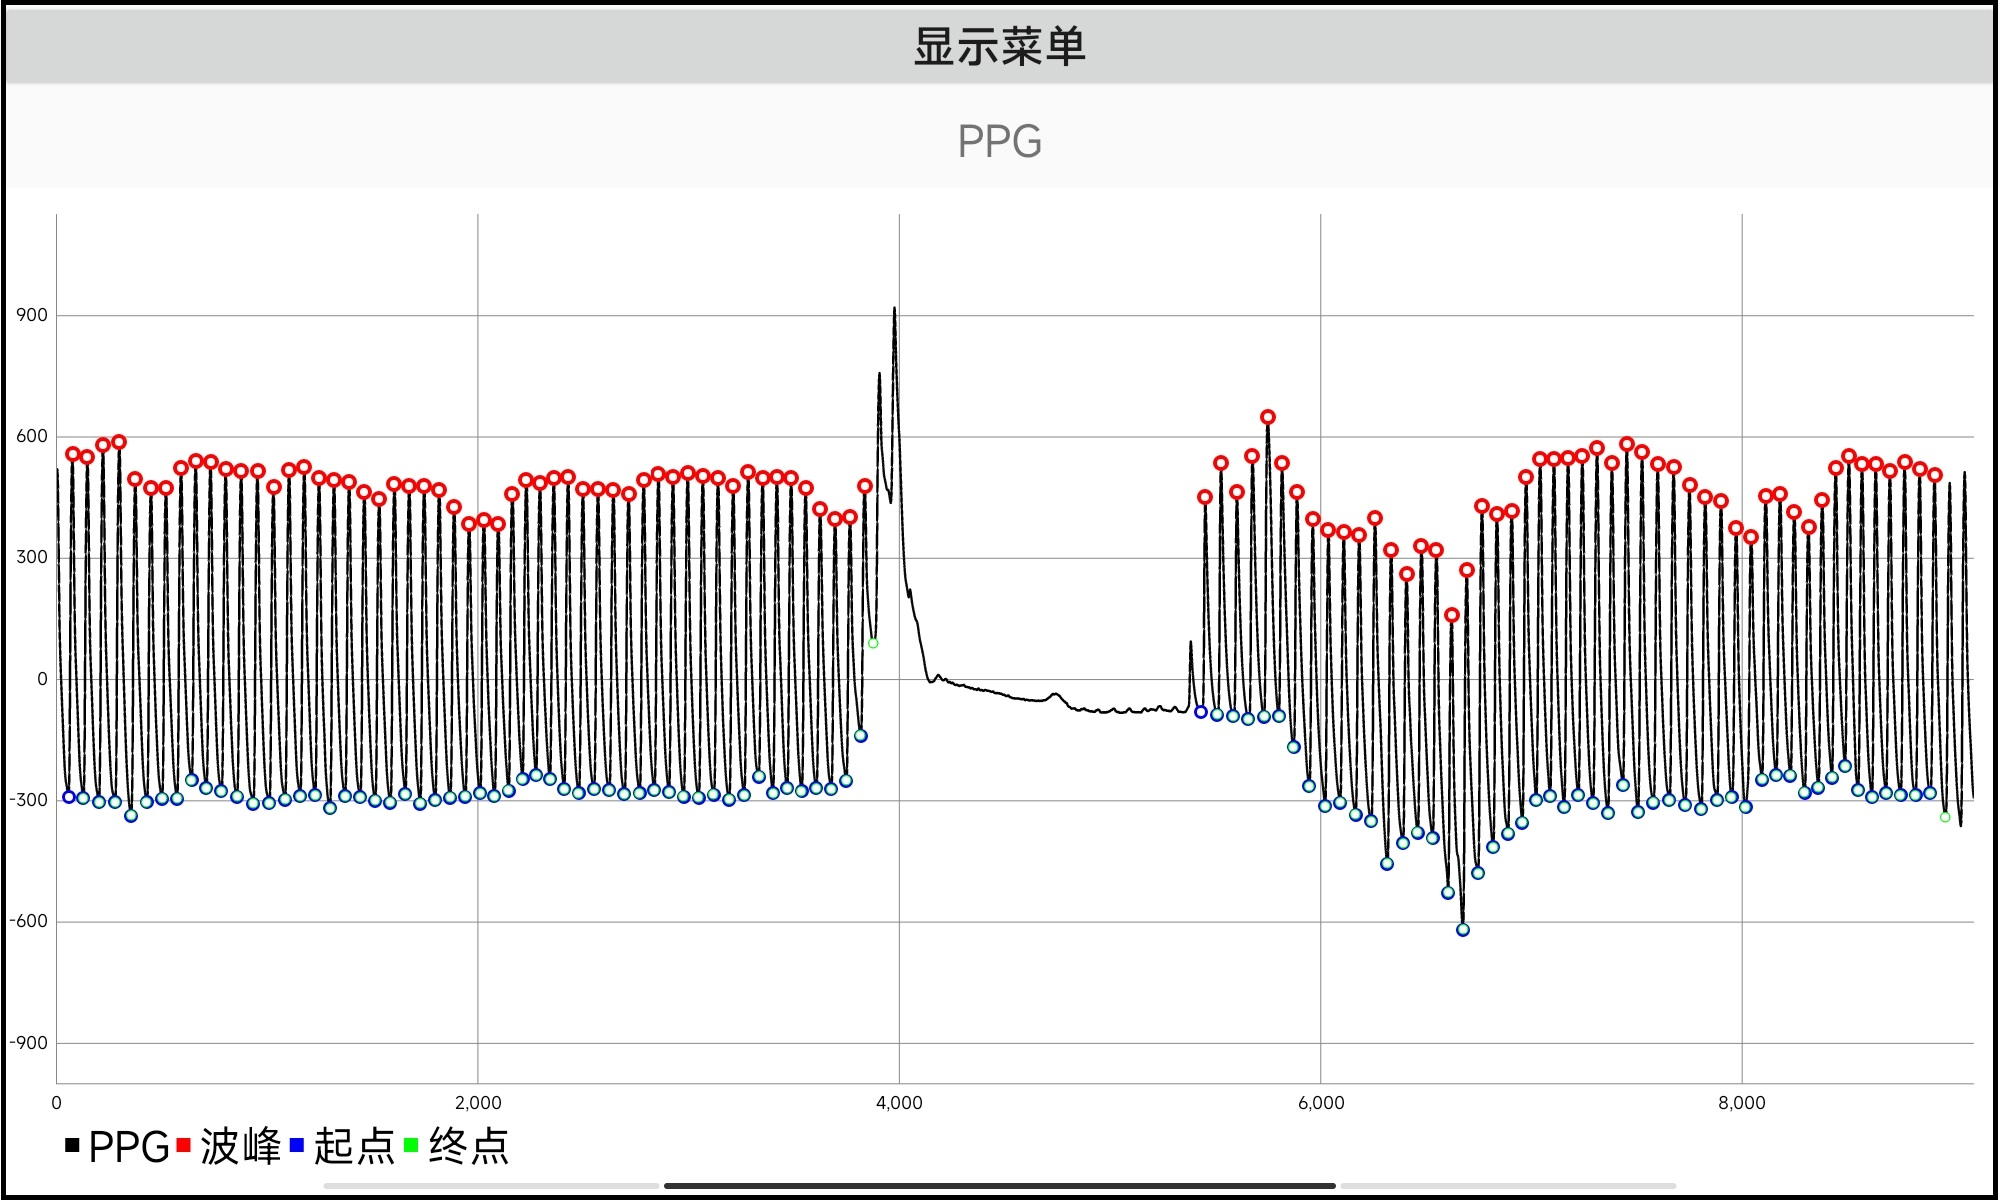
\includegraphics[width=12.65cm]{software/android}
    }
    \quad
    \subfigure[菜单唤出界面]{
    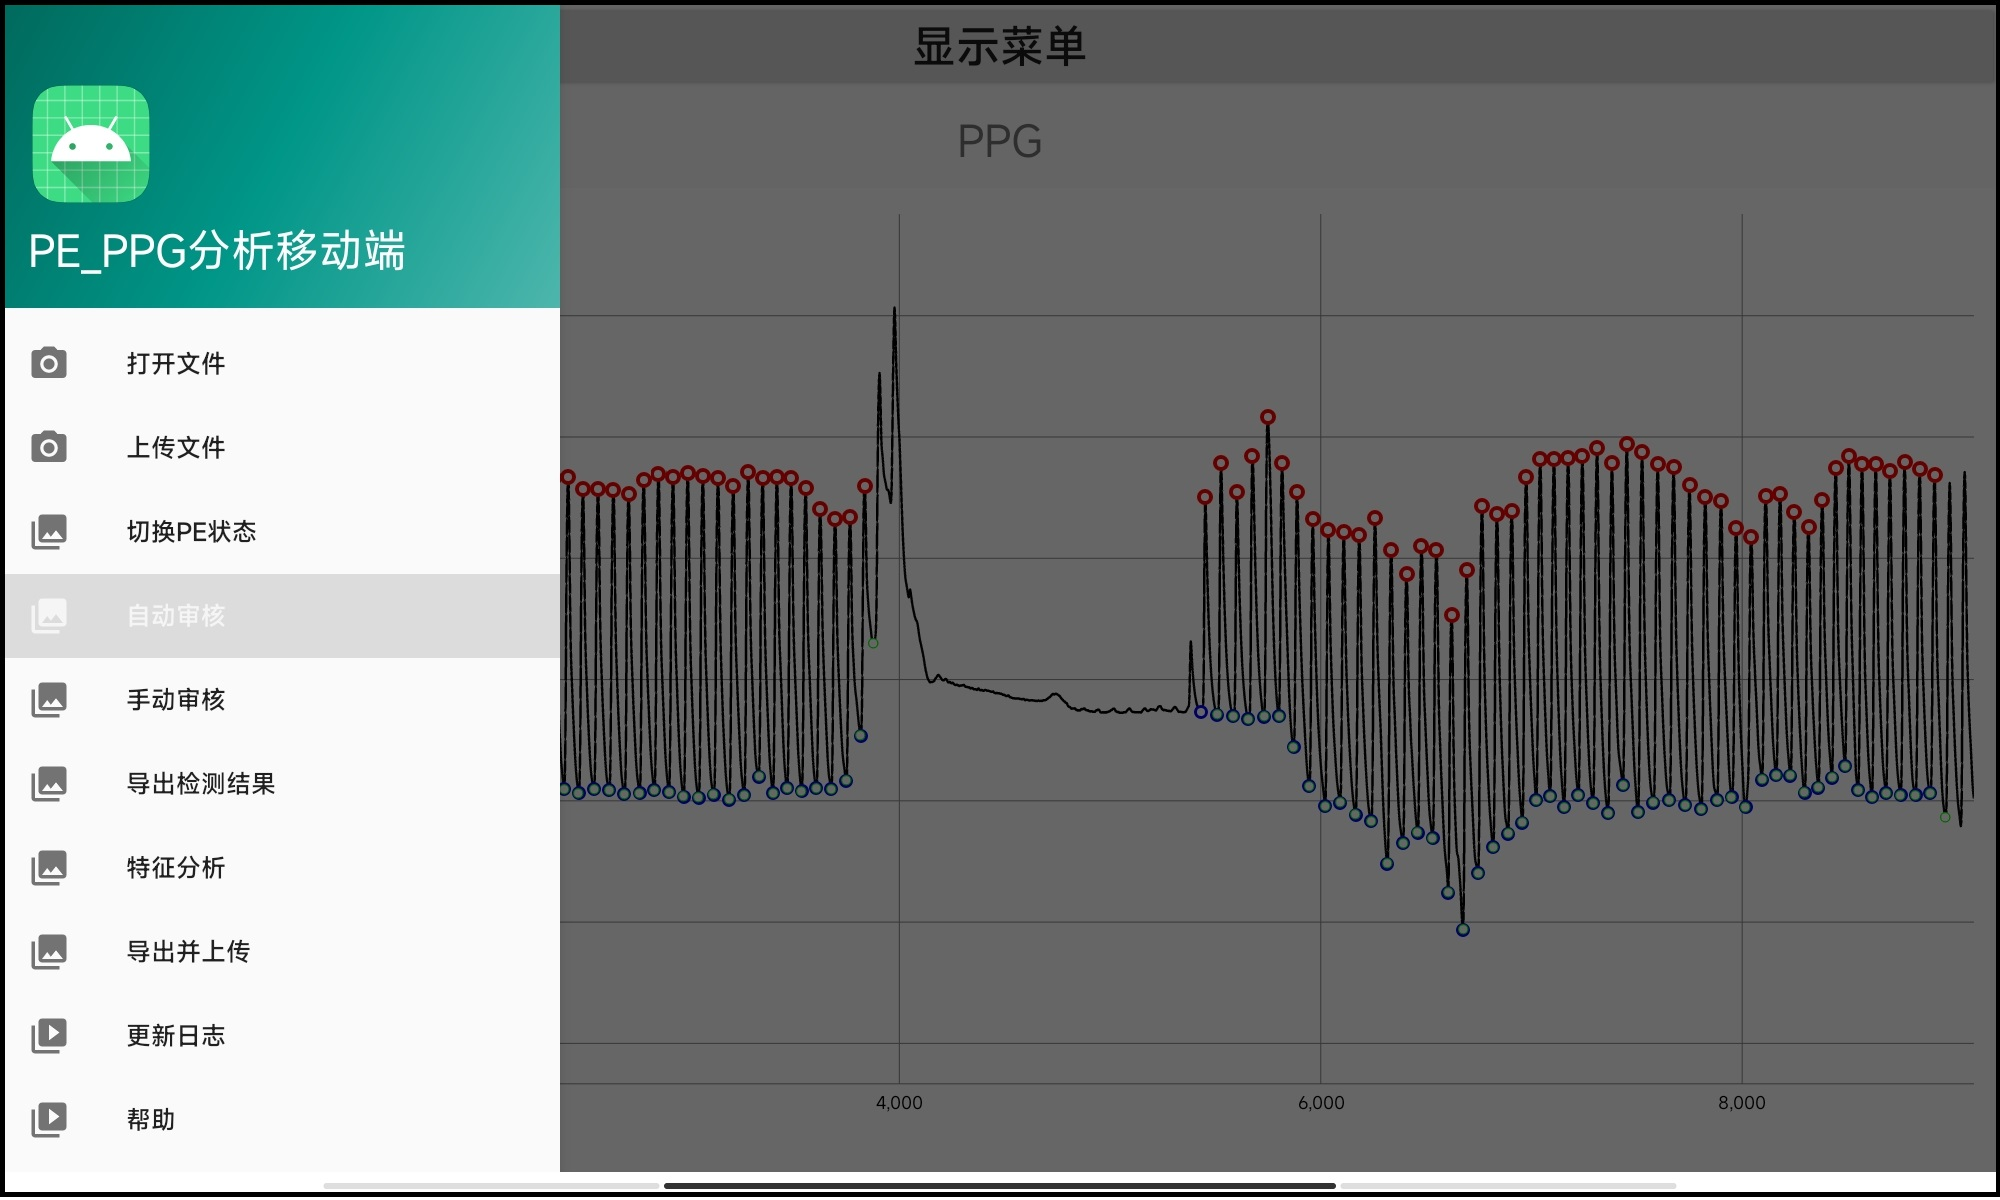
\includegraphics[width=12.65cm]{software/android_menu}
    }
    \caption{\label{fig:android_ui}Android客户端运行界面图}
\end{figure}

\autoref{fig:android_ui}展示了软件分析系统在Redmi Pad SE上运行效果。为充分利用Pad显示界面,菜单栏默认隐藏,需要使用时可点击按钮唤出。
考虑到Android客户端的实际使用场景的差异,上文介绍的PC客户端特色功能暂时未在Android客户端下实现。
但除此之外,Android客户端与PC客户端整体功能相近、操作类似,故此处不再赘述。

\subsection{PE识别模型训练生成模块}
PE识别模型训练生成模块是软件系统的算法核心,负责利用多种机器学习算法基于数据特征完成PE识别模型的训练。在对模型进行一定的评估后,
综合性能表现好的模型才会被部署至云服务端,供PC客户端与Android客户端调用并进行新数据的识别预测。由于Python在机器学习领域的广泛普及应用,
此模块的编程设计全部基于Python实现。

一、数据合并

跨平台客户端程序会把检测得到PPG波形数据与PPG时域特征分别以JSON文件的形式保存至本地并上传至云服务器。此前已经介绍过,JSON文件对数据特征的存储是逻辑上的“树”,
为从多棵这样的数据树中构建出完整的特征数据集矩阵,显然需要一个数据合并的过程。
这就是第四章的脉搏波多维度时域特征集(PMTFS)与脉搏波采样序列时域特征集(PSTFS)的生成过程。
\begin{figure}[htbp]
    \centering
    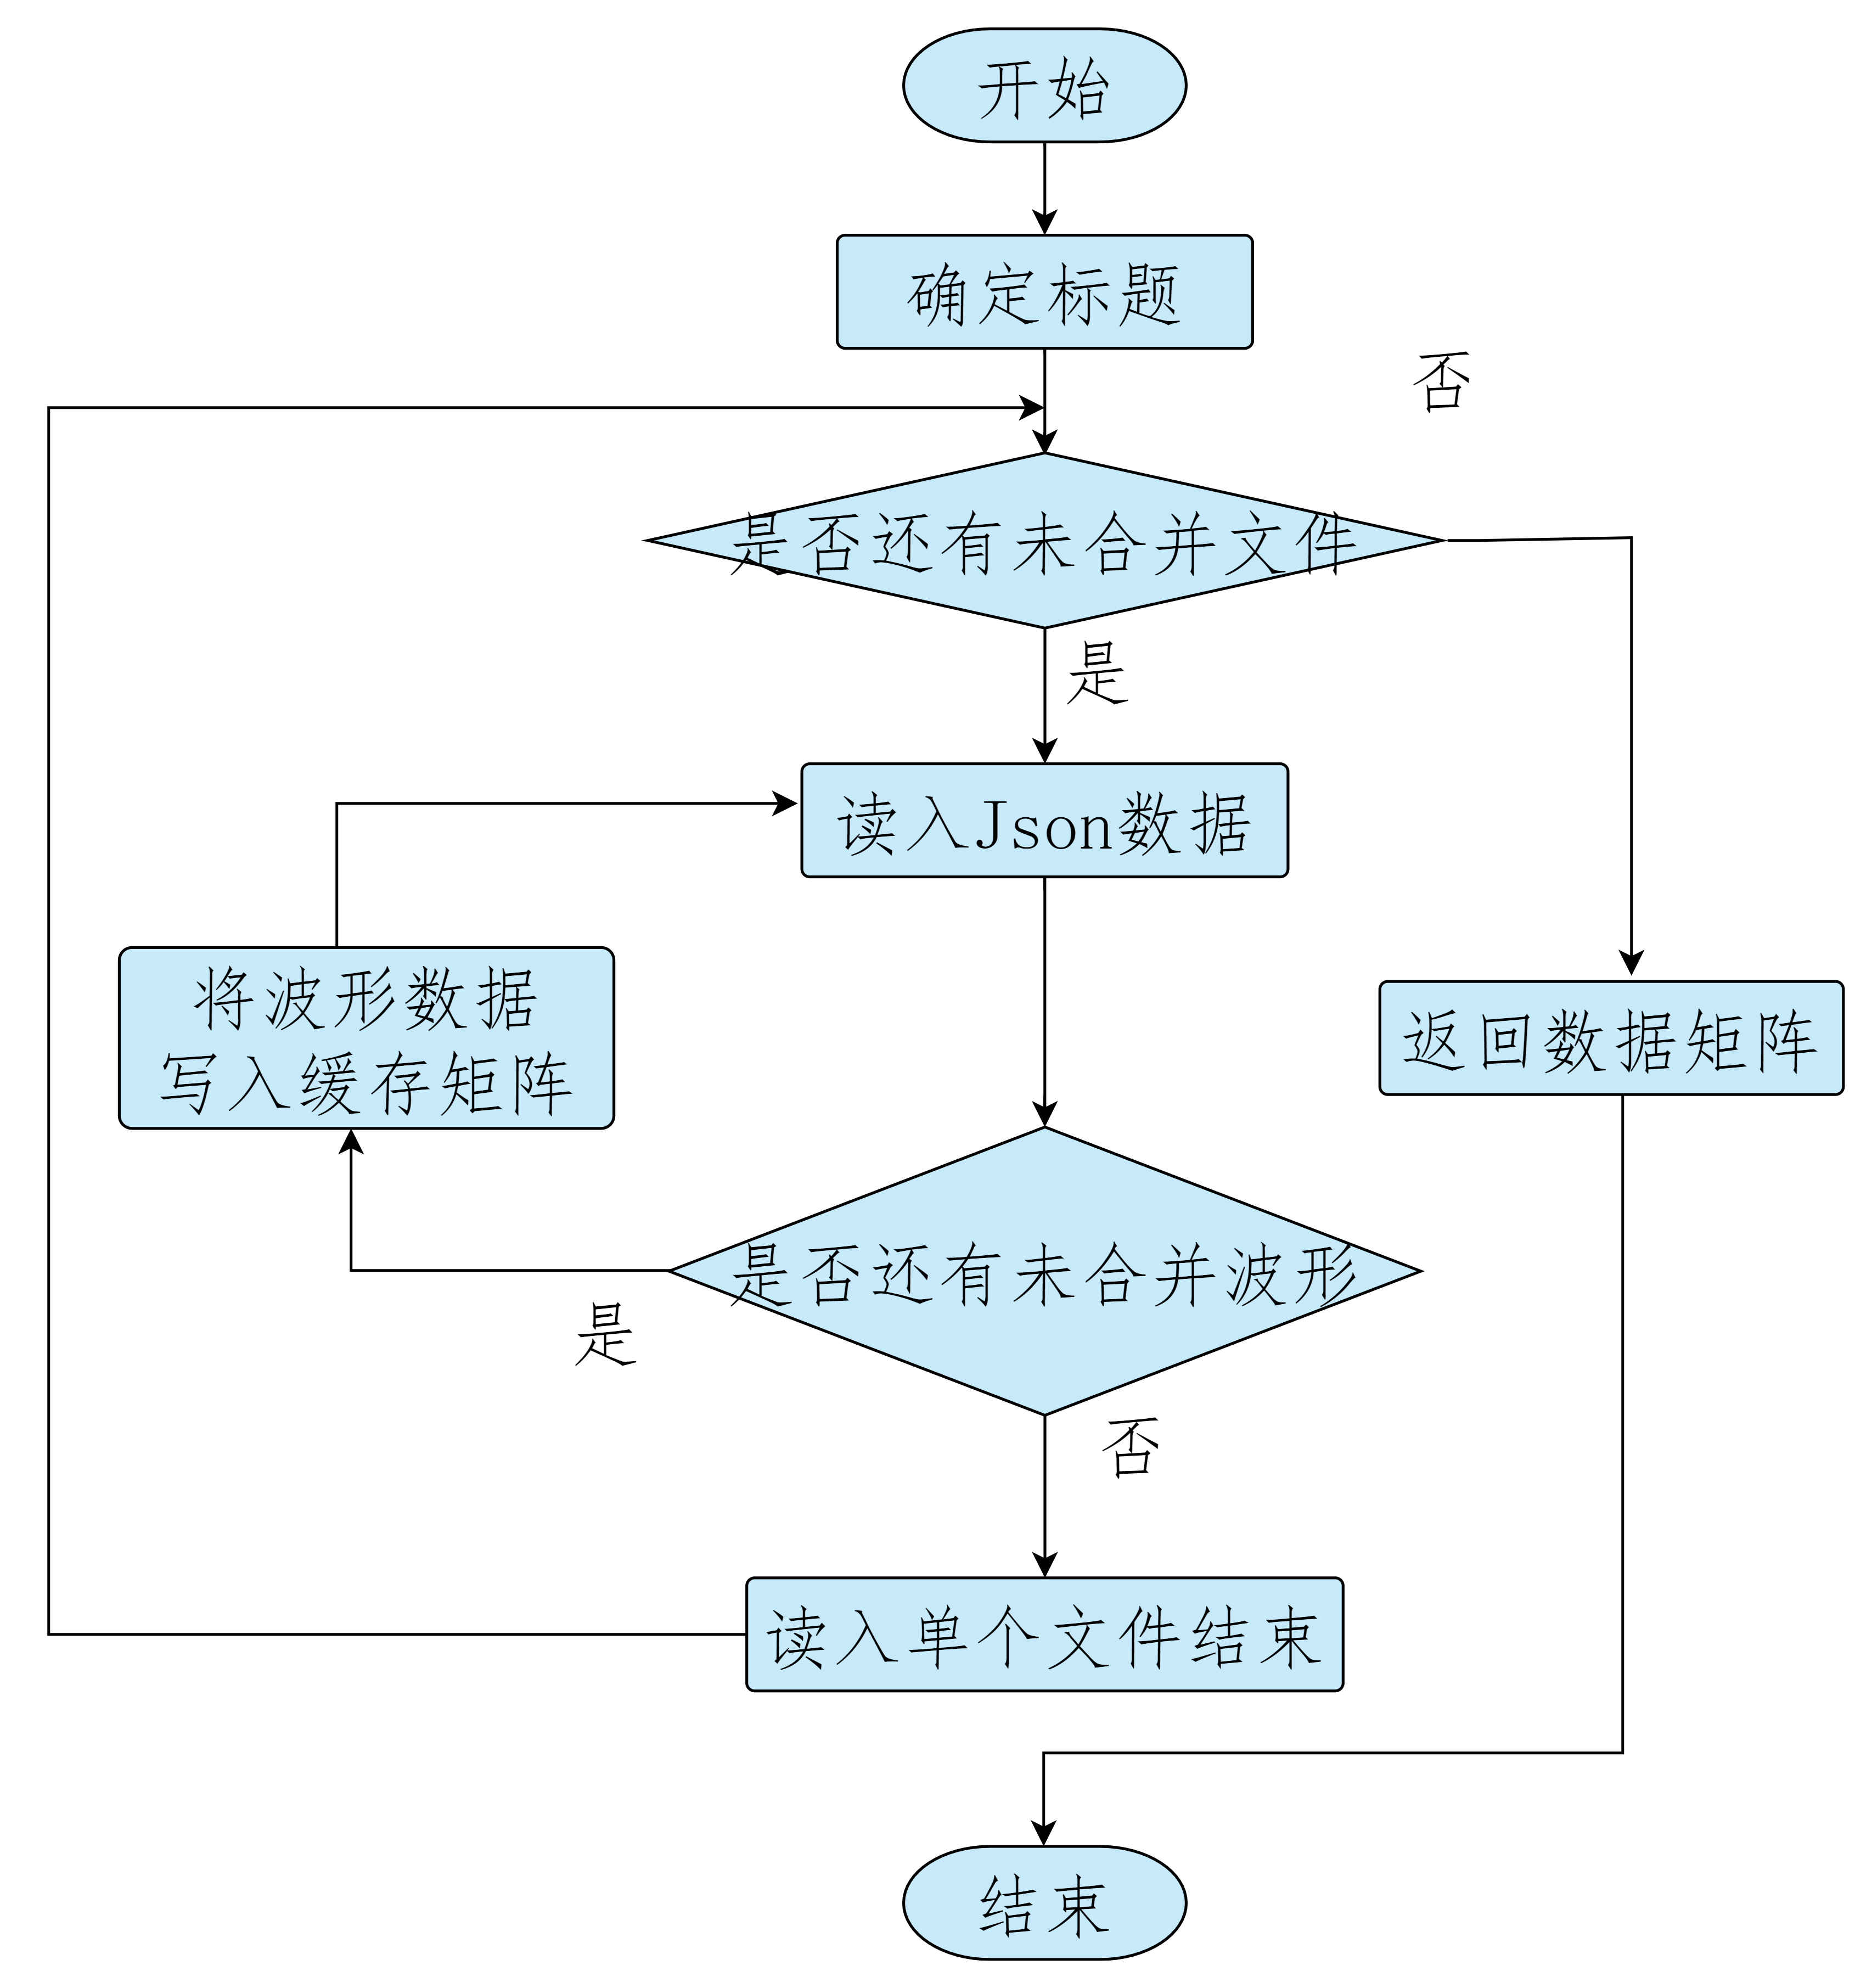
\includegraphics[width=.55\linewidth]{software/mergedata}
    \caption{\label{fig:mergedata}数据合并流程图}
\end{figure}

模块对数据合并的处理流程如\autoref{fig:mergedata}所示。依次读取需要合并的数据特征文件,确定生成矩阵的标题栏,记录下包括软件版本号、原始PPG数据文件名、数据患者名、PE状态等基本信息,
随后开始记录数据特征文件的所有特征数值,PPG波形序号也被同时记录。而当生成PSTFS时,需要根据PPG波形对齐策略的选择,将原始采样值量化至指定区间内。
按此方式依次处理完所有文件即可得到包含最终的数据集矩阵的CSV格式文件。

二、数据划分

为使由不同机器学习算法训练所得的PE识别模型的性能具有可比性,需要通过控制变量法,让所有的机器学习算法在相同的训练数据集上训练模型,并在相同测试
数据集上评估性能。
\begin{figure}[htbp]
    \centering
    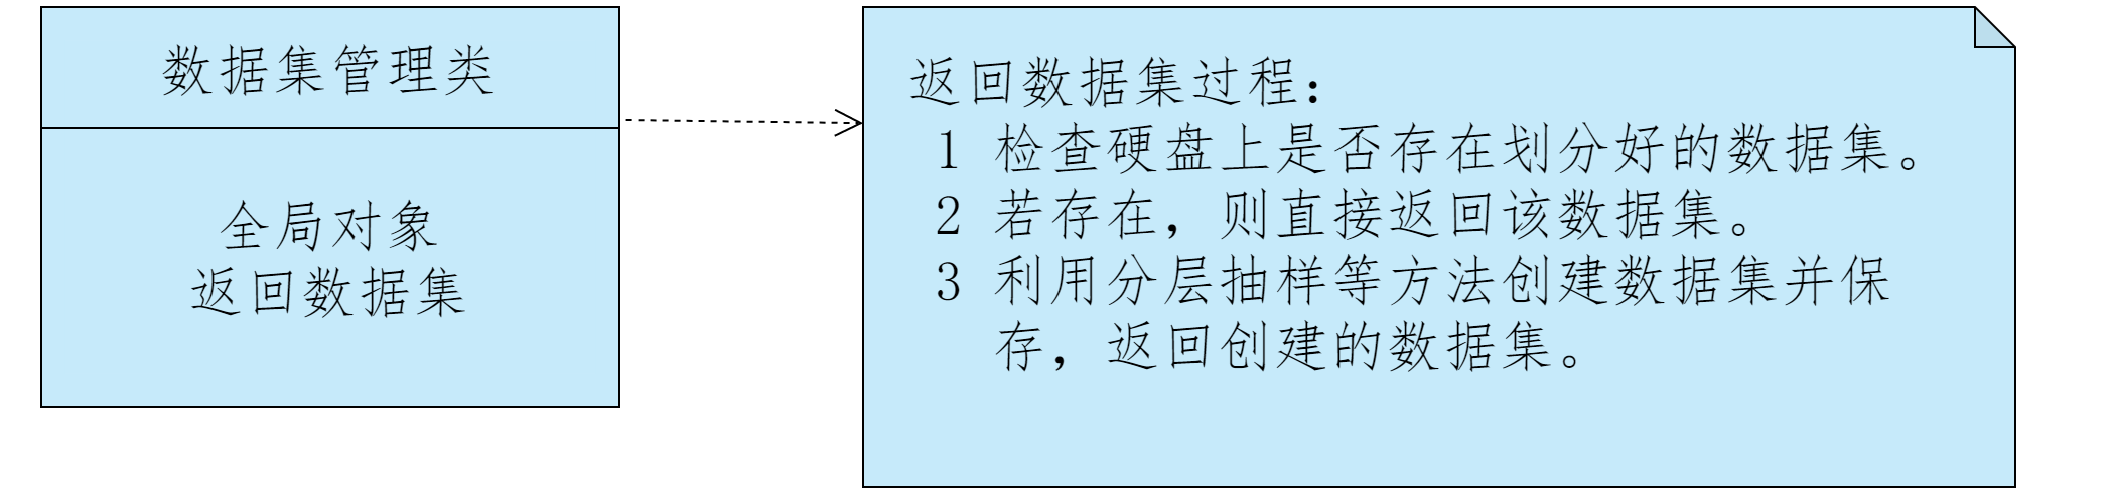
\includegraphics[width=.8\linewidth]{software/loaddataset}
    \caption{\label{fig:loaddataset}数据集划分创建过程示意图}
\end{figure}

本模块对数据划分的流程如\autoref{fig:loaddataset}所示。一个单独的数据集管理类负责返回所有模型所需的训练集数据与评估测试集数据,而在该类内部,每当接收到数据集读取请求时,
函数都会先去检查硬盘上是否已有划分好的数据集。
如果存在这样的数据集,则直接读取硬盘上数据集并返回;否则,函数会调用数据集分层抽样等函数并生成特定的数据集,将该数据集保存至硬盘上后返回该数据集。
对比数据预处理模块的特征计算的\autoref{fig:singleton}可以发现,这种数据集划分方式也可以视为一种广义上的单例程模式,区别在于后者多了一次对硬盘数据的检查和读取。

三、模型训练与保存

机器学习的过程一般包括载入数据、在训练集上进行训练、考察训练集上的性能、在测试集上测试等操作,其中的某些步骤更涉及到多个参数的计算与比较。
在PE识别模型的构建过程中,由于涉及多个模型的比较,需要不断重复上述操作,该过程繁琐且极易疏漏。
另一方面,由于PE识别模型均是借助Python下Sklearn工具包完成的\cite{scikit-learn},而Sklearn本身在设计过程中均遵循了统一规范,不同的机器学习算法均提供了相同的API函数。
因此,软件系统对PE识别模型的构建过程额外进行了封装,在实现代码的最小化的同时,也避免了算法模型训练过程的代码遗漏等问题,同时也简化了模型训练过程。

软件系统中将模型训练过程封装成了MyClasssifer类,该类一共包含四个可调用的公开函数:
$init()$、$load\_data()$、$fit\_predict()$与$grid\_search()$。其中,$init()$函数为MyClasssifer类新建实例初始化函数,入口参数为Sklearn中的机器学习算法实例;
$load\_data()$函数调用上述数据集管理类,负责载入训练集与测试集数据;$fit\_predict()$函数封装了机器学习算法在训练集与测试集上的全部处理操作;而
$grid\_search()$为模型超参数探索时的网格化搜索函数。
特别地,在$fit\_predict()$函数中集成封装了Sklearn工具包中各算法模型的多项重要函数,其处理流程如\autoref{fig:fit_predict}所示。
在\autoref{fig:fit_predict}中,为使模型可复现,$fit\_predict()$函数在保存生成的模型的同时也将训练该模型的所需的超参数进行了保存。

\begin{figure}[ht]
    \centering
    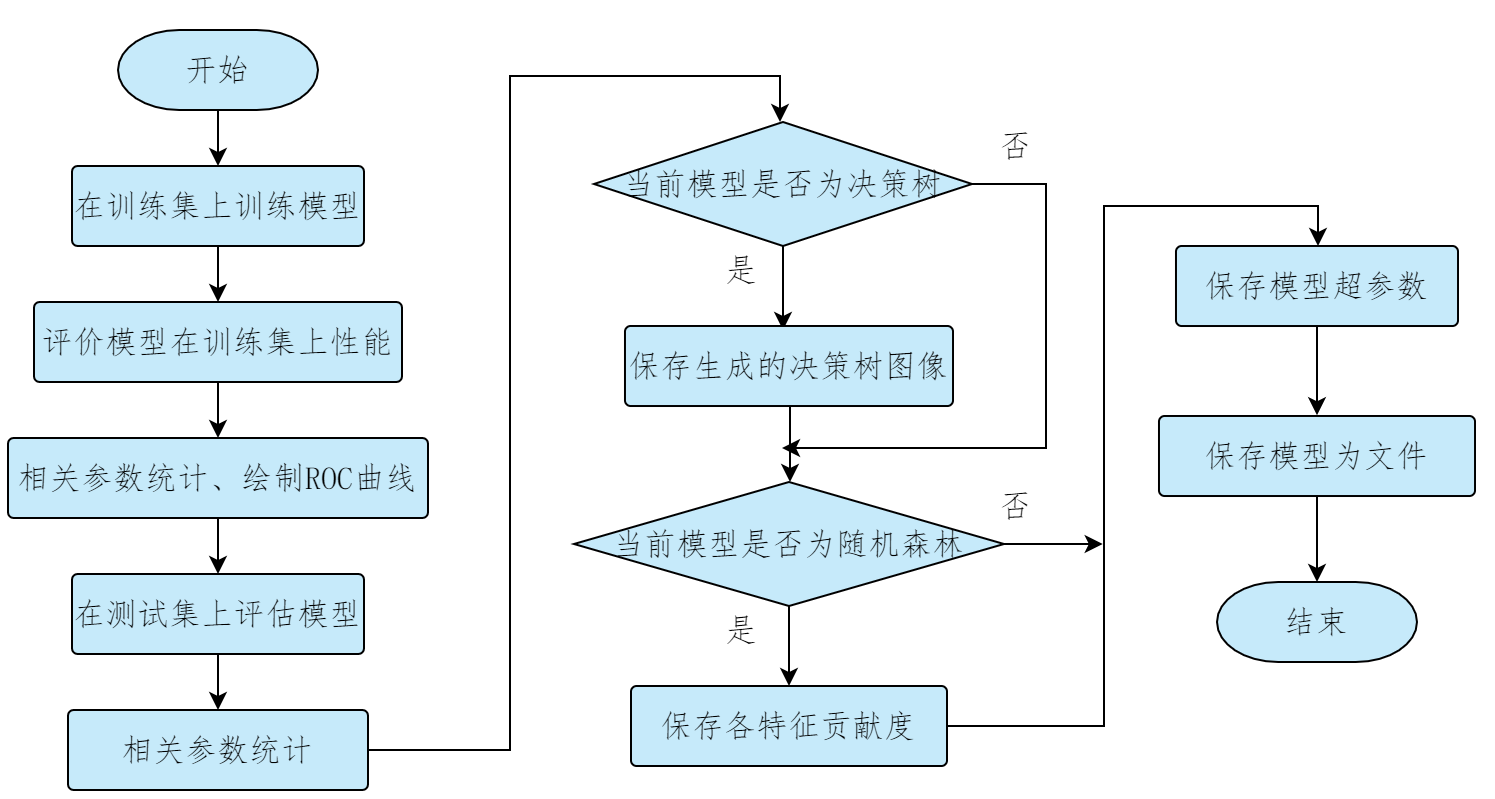
\includegraphics[width=\linewidth]{software/fit_predict}
    \caption{\label{fig:fit_predict}封装后的$fit\_predict()$函数处理流程图}
\end{figure}

四、日志记录

与此前的客户端程序类似,为方便调试与记录模型训练过程中的各项参数与中间变量等信息,模型训练模块也利用Python下的logging包\cite{logging}开发了程序日志记录功能。


\subsection{云服务器模块}
当云服务器端接收来自客户端的特征数据猴,在进行数据校验确认无误后,所有原始数据都会被保存至数据库中。
随后,会根据客户端的请求内容,选择一个或多个已经存储在云服务器端的机器学习模型进行新数据的识别预测,并将结果返回至客户端。


一、网络协议选择与数据接口设计

为使客户端软件与云服务器端能够进行数据通信与数据交换,软件系统选择了最为常见的超文本传输协议(hypertext transfer protocol,HTTP)\cite{http}。
HTTP是一种简单的请求——响应协议,它指定了客户端可能发送给服务器的消息类型以及能得到何种响应,通常运行在TCP协议之上。

1、POST与GET

一般而言,一个统一资源定位器(uniform resource locator,URL)地址描述了一个网络资源。而HTTP协议中定义的PUT、DELETE、POST与GET等与服务器进行交互的基本方法,
对应着对该网络资源的增、删、改、查等基本操作\cite{http}。
其中,GET方法与POST方法均能向服务器端传递数据,在互联网应用中使用的最为广泛。
由于POST方法较GET方法功能更为强大,能够同时传递文本数据与二进制文件数据,因而被选为软件系统的客户端与云服务器端的默认通讯方法,如\autoref{tab:get_post}所示。

\begin{longtblr}
    [
        theme                   = {zju},
        caption                 = {GET方法与POST方法对比},
        label                   = {tab:get_post},
    ]
    {
        width                   = \linewidth,
        colspec                 = {X[1,c,m]X[3,c,m]X[3,c,m]},
        hline{1,Z}              = {\thickline},
        hline{2}                = {\thinline},
        rowhead                 = 1,
        row{1}                  = {font=\headfont},
        row{2-Z}                = {font=\nonheadfont},
    }
    &GET&POST\\
    常用场景&获取、查询信息&更新资源信息\\
    数据传递方式&请求参数与数值附加在URL后&封装在HTTP请求中\\
    传递数据量&受限,一般为1024个字符&无限制\\
    编码方式&只允许ASCII字符&没有限制,也允许二进制数据\\
    安全性&较差,数据是URL的一部分&较安全,参数不会被记录保存\\
\end{longtblr}

2、POST方法的参数设计

客户端程序通过POST方法向云服务器端提交数据的通讯过程中涉及到的所有参数如\autoref{tab:post_paras}所示。
\vskip 20pt
\begin{longtblr}
    [
        theme                   = {zju},
        caption                 = {客户端在POST方法中上传参数},
        label                   = {tab:post_paras},
        note{*}                 = {文件类型数据。},
    ]
    {
        width                   = \linewidth,
        colspec                 = {X[1.5,c,m]X[3,c,m]X[1,c,m]X[1,c,m]X[2.5,c,m]},
        hline{1,Z}              = {\thickline},
        hline{2}                = {\thinline},
        rowhead                 = 1,
        row{1}                  = {font=\headfont},
        row{2-Z}                = {font=\nonheadfont},
    }
    参数的键名&参数值的含义&{数据流\\类型}&数据类型&备注\\
    project&上传的数据归属的具体项目&文本&字符串&{值固定为PE,代表数据隶属本论文基于PE的研究}\\
    data\_type&上传的数据所属生理信号类别&文本&字符串&{值固定为PPG}\\
    client&上传数据的客户端类型&文本&字符串&值为PC或Android\\
    version&上传数据的客户端程序版本号&文本&字符串&不同客户端软件版本号可能不同\\
    algorithm\_version&数据预处理模块的算法版本号&文本&字符串&不同客户端算法版本可能不同\\
    person&上传数据对应的孕妇名&文本&字符串&{遵循医学伦理学相关标准,省略孕妇具体姓名,仅以拼音缩写代替}\\
    pe\_state&上传数据对应孕妇的PE状态&文本&整型&0为健康孕妇,1为PE患者,2为待定\\
    source&此次上传对应的原始PPG文件名&文本&字符串&\\
    source\_file\TblrNote{*}&此次上传对应的原始PPG文件数据&文件&文件数据&按二进制编码成数据流发送\\
    feature\_file\TblrNote{*}&基于原始PPG数据计算得到的特征数据&文件&文件数据&按二进制编码成数据流发送\\
    point\_file\TblrNote{*}&基于原始PPG数据计算得到的波形采样值数据&文件&文件数据&按二进制编码成数据流发送\\
    sample\_time&原始数据的采集时间&文本&字符串&{可选项,本论文中由于导出数据包含数据采样时间,故增设该值}\\
    predict&本次上传的数据是否需要进行预测分析&文本&字符串&值为True或False\\
    model&本次上传数据分析所使用的机器学习模型&文本&字符串&值为具体机器学习算法模型\\
    upload\_time&本次通信上传时间&文本&字符串&\\
\end{longtblr}

二、模型的上传

在PE识别模型训练完成之后,所得模型也需要被上传部署在云服务器端。为使机器学习模型的部署更为便捷、清晰,软件系统也基于Python的图形界面PyQt额外开发了
机器学习模型上传程序\cite{pyqt,zhiyiYo2023},在上传时需将包括使用的算法、训练集、版本号等信息一并提交。%,如\autoref{fig:upload_model}所示。

三、基于Django的服务器端程序设计

由于本研究涉及的所有机器学习模型均是通过Python下的Sklearn包生成,为方便调用,软件系统最终选取了同样基于Python的开源通用Web框架Django进行相关云服务器端的功能开发\cite{django}。
Django按模型-模版-视图(model template view,MTV)设计模式的进行了整体结构设计\cite{django},如\autoref{fig:django}所示。
\begin{figure}[htbp]
    \centering
    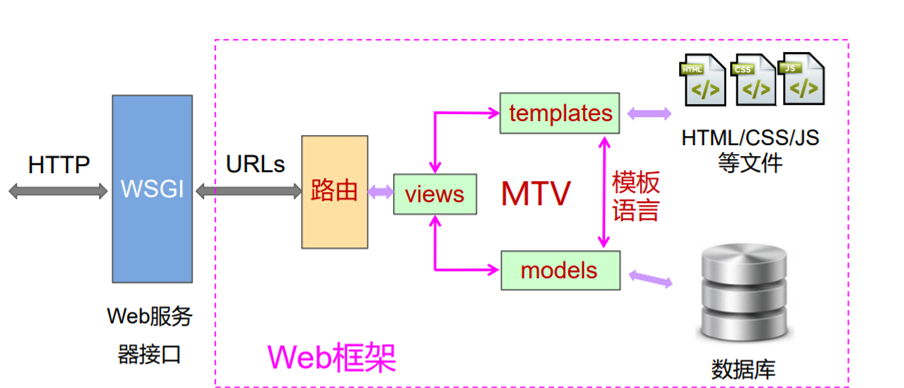
\includegraphics[width=.75\linewidth]{software/django}
    \caption[Django框架结构示意图]{\label{fig:django}Django框架结构示意图}
\end{figure}

1、处理流程

云服务器端的程序处理流程实际上对应着\autoref{fig:django}中的视图,即业务逻辑层。当云服务器端接收到客户端的数据请求或模型上传请求时,云服务器端程序会依据请求对应的不同
URL路由地址,选择对应的处理流程,这一过程如\autoref{fig:url}所示。

\begin{figure}[h]
    \centering
    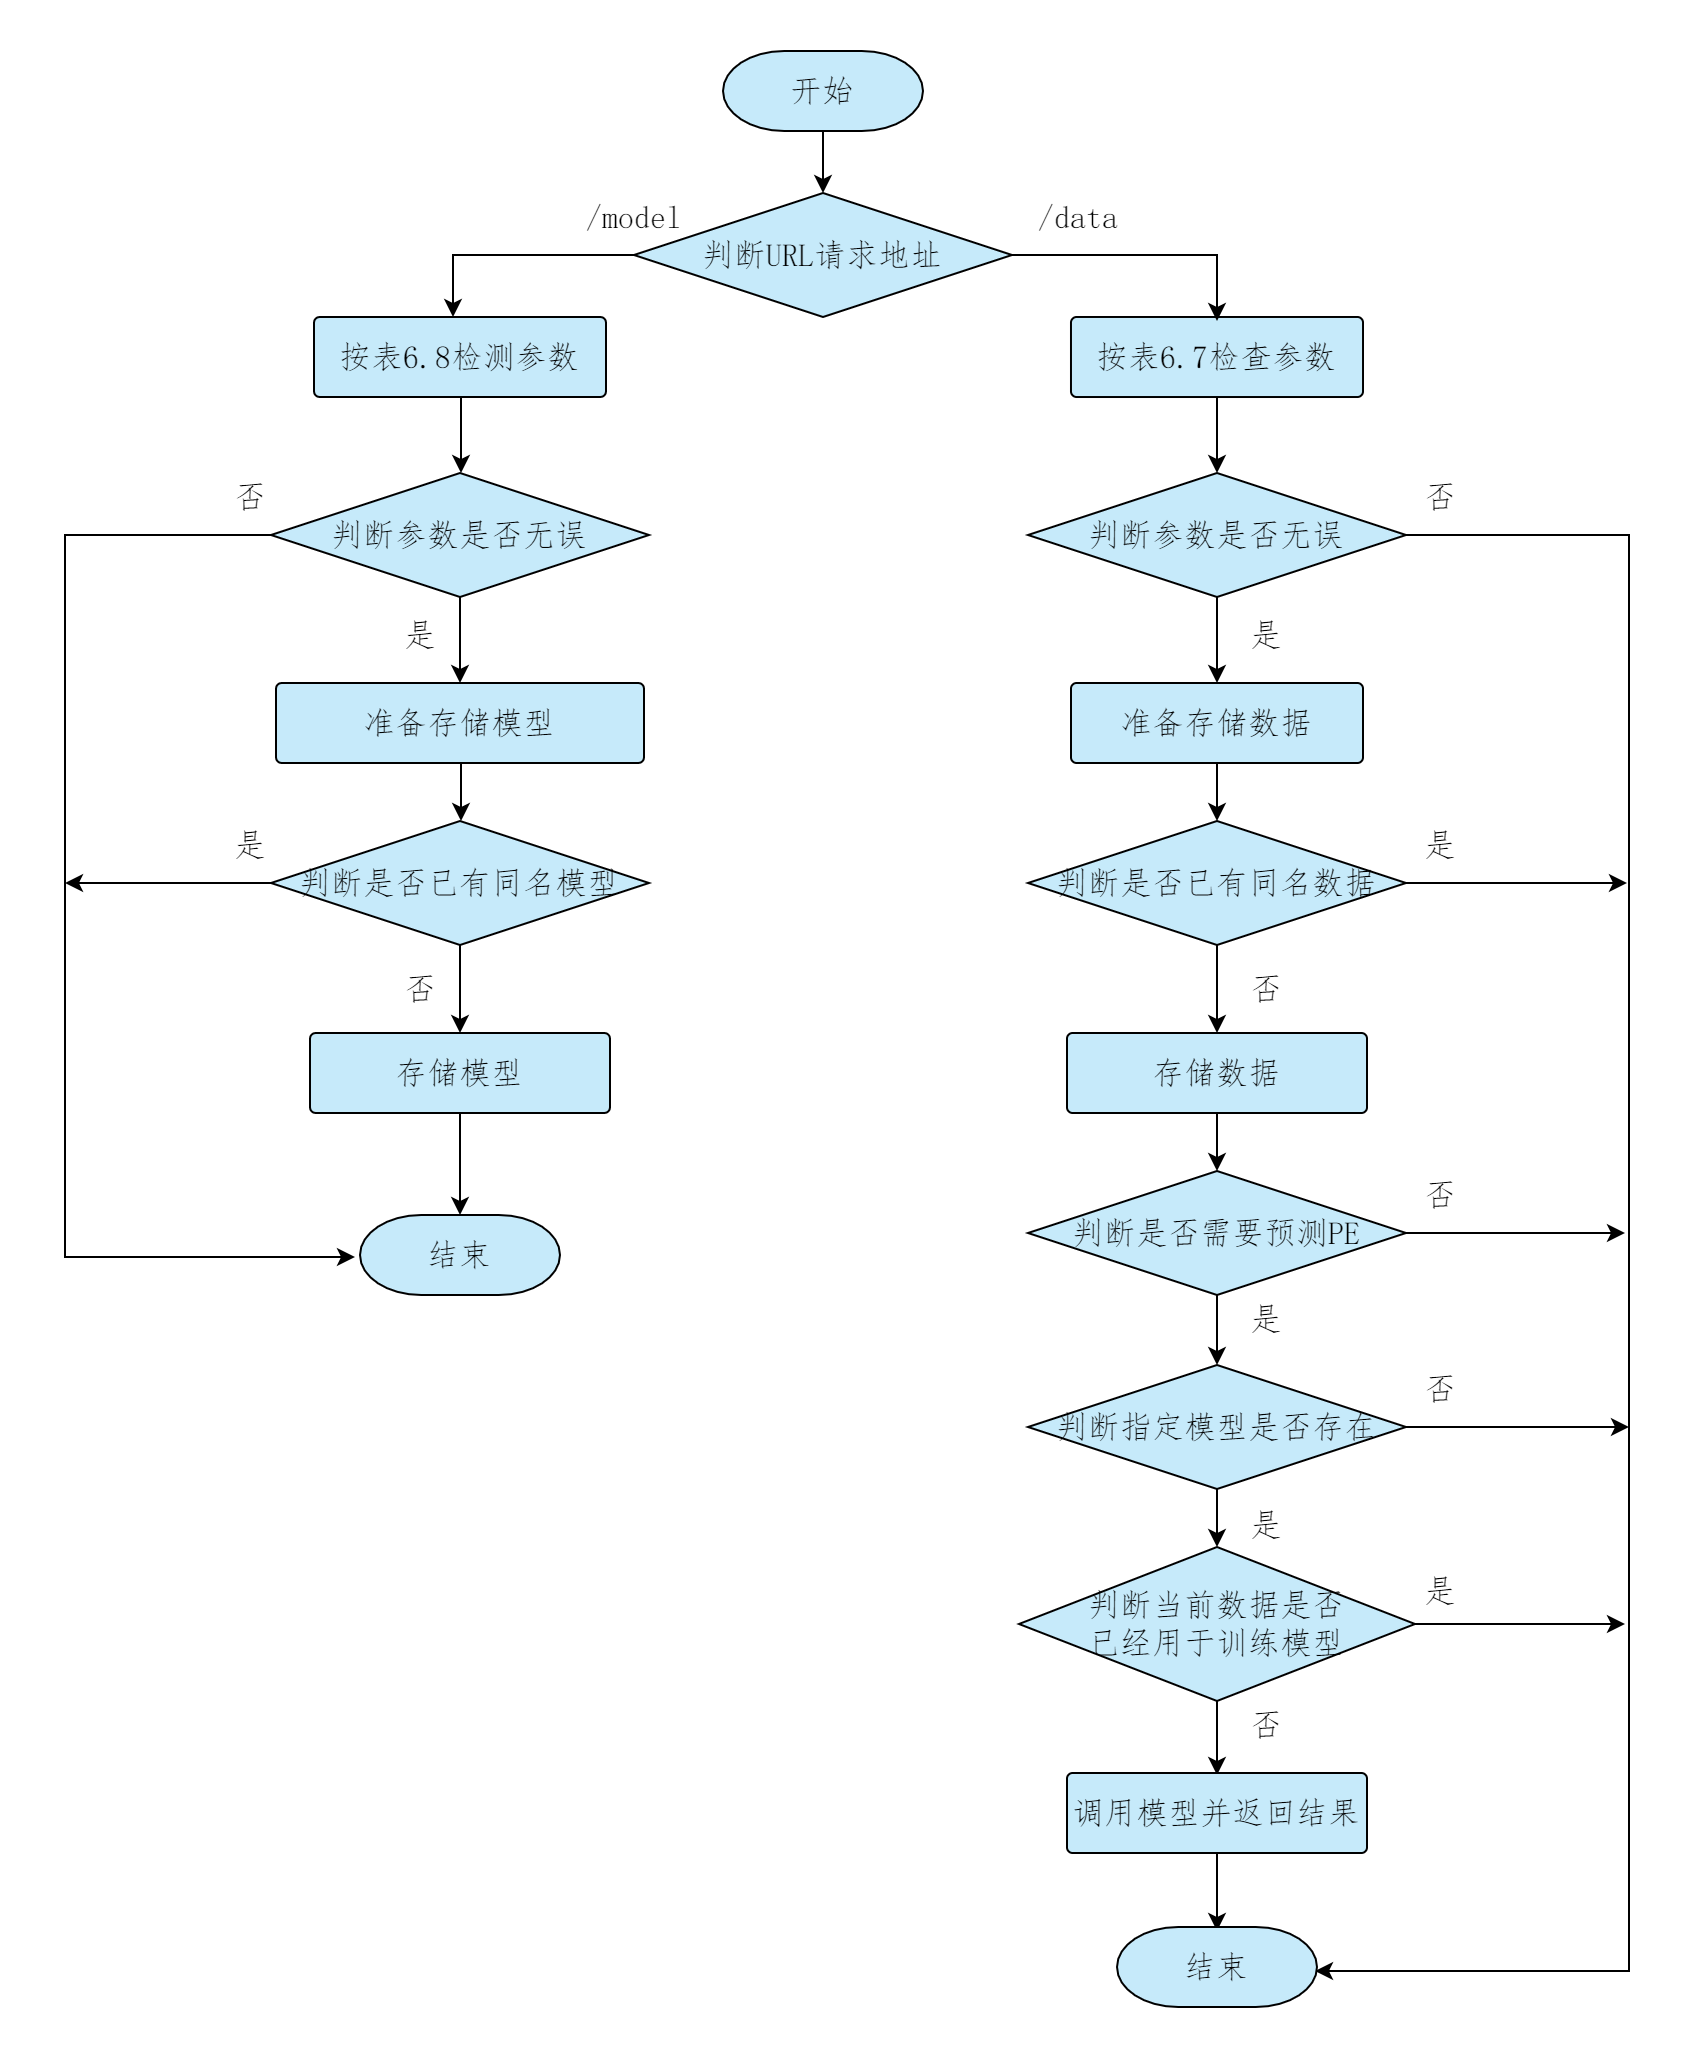
\includegraphics[width=\linewidth]{software/url}
    \caption{\label{fig:url}云服务器响应URL请求过程流程图}
\end{figure}

2、模型与数据库

\autoref{fig:django}中的模型涉及了数据库的处理操作,这部分的程序设计会在后续进行介绍。

3、日志

为方便调试,云服务端在使用Django进行开发时,也使用了Python下的logging包进行日志记录功能开发\cite{logging}。

四、数据库设计

软件系统选择了目前流行的主流关系数据库之一的MySQL进行相关数据的存储\cite{mysql}。MySQL遵循结构化查询语言(structured query language,SQL)标准,支持查询、新增、更新、删除、求和、排序等基本操作。与此同时,软件系统一共设计了五张数据表(Table)来解决上述问题。这些数据表之间的相互关联关系如\autoref{fig:data_table_relationship}所示,各数据表的重要的外部键也在图中进行了标注。
\begin{figure}[htbp]
    \centering
    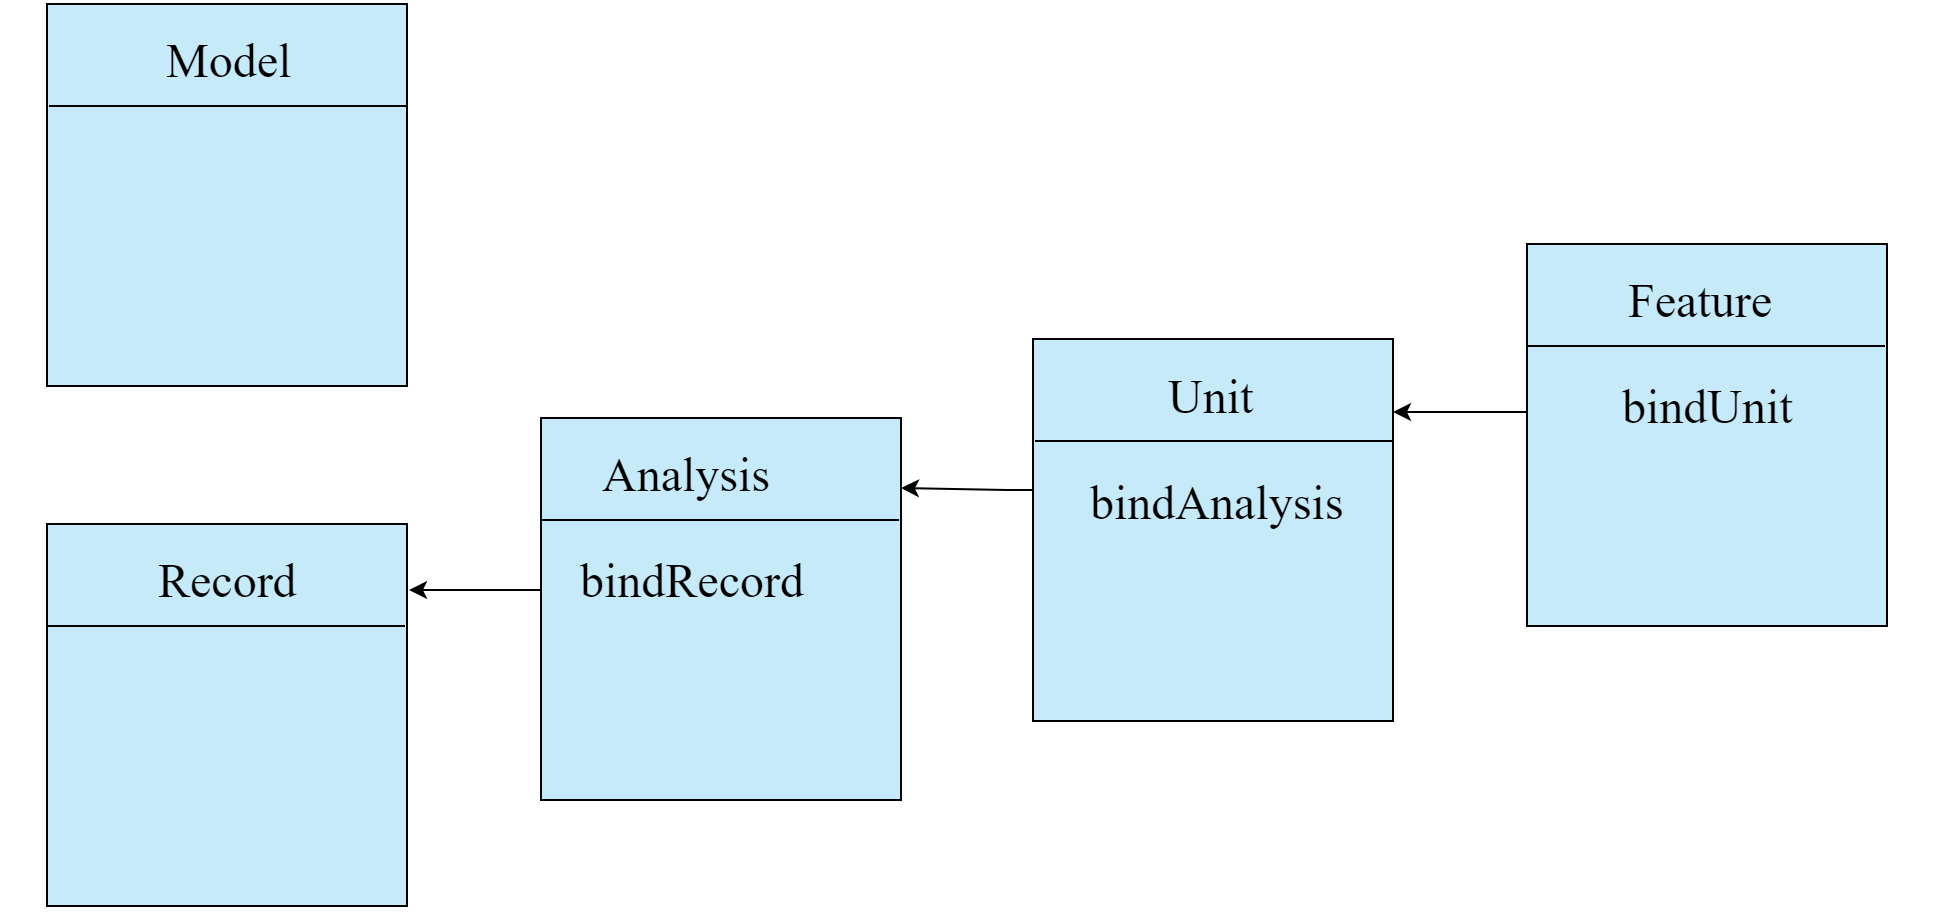
\includegraphics[width=.75\linewidth]{software/data_table_relationship}
    \caption{\label{fig:data_table_relationship}软件系统的数据表及数据关系示意图}
\end{figure}

从\autoref{fig:data_table_relationship}可以看到,软件系统中PE识别模型的存储过程较为简单,只需一张数据表;而生理信号数据及其衍生特征的存储较为复杂,需要四张数据表级联并相互配合。
其中,Model数据表维护了所有分析模型信息;Record数据表维护了所有数据记录信息;Analysis数据表维护了所有数据文件信息;Unit数据表维护了所有最小分析单位信息;而
Feature数据表维护了所有PPG特征信息。下面以Feature数据表为代表详细介绍数据表的设计。

\begin{longtblr}
    [
        theme                   = {zju},
        caption                 = {Feature数据表的字段设计},
        label                   = {tab:data_table_feature},
    ]
    {
        width                   = \linewidth,
        colspec                 = {X[1,c,m]X[2,c,m]X[3,c,m]X[4,c,m]},
        hline{1,Z}              = {\thickline},
        hline{2}                = {\thinline},
        rowhead                 = 1,
        row{1}                  = {font=\headfont},
        row{2-Z}                = {font=\nonheadfont},
    }
    字段&数据类型&意义&备注\\
    id&32位整型&自增字段&主键,随记录存储自动增加\\
    bindUnit&Analysis数据表中的Unit记录&当前记录绑定的Unit数据表记录ID&关联到Unit数据表的外部键\\
    type&字符串&操作标记&兼容性设计,在PE项目组,对PPG的特征类数值无意义;对PPG的采样点数据记录的均一化等特性\\
    name&字符串&特征数据名称&兼容性设计,特征名。在PE项目组,特征类数据该值为具体特征缩写;对采样点数据该值固定为point\\
    value&JSON&具体特征值&兼容性设计,Django支持直接以JSON形式存储字段信息\\
    isDeleted&布尔量&当前记录是否被逻辑“删除”&为避免记录被直接物理删除,额外增加的布尔变量指代是否被删除状态\\
\end{longtblr}

Feature数据表存储了对PPG记录的单个波形的所有特征,而bindUnit字段是关联到Unit数据表的外部键,如\autoref{tab:data_table_feature}所示。
特别地,PPG时域特征与原始采样值序列都可以直接以JSON格式存储在value字段中,只需通过name字段进行区分即可,其中前者的name字段数值
多变,而后者固定为point。另外,对原始采样值而言,可能存在均一化、滤波等操作,这些操作的差异被存储入type字段。最后,数据表中额外增加了isDeleted字段用以处理数据记录的删除,当需要删除
数据时,只需更改该字段的布尔值,避免了物理删除彻底丢失对数据后续管理的可能。

\section{测试与验证}
上文对\autoref{fig:scas}中展示的软件框架的设计与实现细节进行了全面详细的说明。而按照这些设计完成软件系统的整体开发后,
系统各模块单独的功能与模块间的协作等尚需进行一定的验证与测试,本小节将对这部分的工作进行介绍。

\subsection{数据预处理的测试与验证}
数据预处理模块的验证主要集中在对本研究设计提出的SCD波形检测算法的验证与测试上。
基于自采实验数据与标准数据库数据\cite{Kachuee2015,ucibp2022},对SCD算法进行了测试验证。同时,也选取了两种有代表性的PPG检测算法与SCD算法进行了对比验证\cite{Chen2019,van2019,van20192}。

上述多种PPG检测算法之间的对比过程可参见本论文第三章,具体对比结果如\autoref{tab:scd_6}所示。
可以看到本研究提出的SCD算法对PPG波形的识别准确率高、抗干扰能力强,与其他算法相比也具有一定的优势。
\begin{longtblr}
    [
        theme          = {zju},
        caption        = {三种PPG检波算法性能对比统计},
        label          = {tab:scd_6},
        note{*}        = {性能最优。},
    ]
    {
        colspec        = {X[0.9,c,m]X[2,c,m]X[1.9,c,m]X[1.45,c,m]X[0.95,c,m]X[1.45,c,m]X[0.94,c,m]X[1.45,c,m]X[0.95,c,m]},
        hline{1,Z}     = {\thickline},
        hline{3}       = {\thinline},
        rowhead        = 2,
        row{1-2}       = {font=\headfont},
        row{3-Z}       = {font=\nonheadfont},
        cell{1}{1-3}   = {r=2,c=1}{c,m},
        cell{1}{4,6,8} = {r=1,c=2}{c,m},
    }
    序号 & 数据源 & 波形总数/个 & SCD算法 & & DMTW算法\cite{Chen2019} & & HeartPy算法\cite{van2019,van20192} & \\
    &  &  & 错检数/个 & 准确率 & 错检数/个 & 准确率 & 错检数/个 & 准确率  \\
    1 & 自主实验数据 & 7864 & 26 \TblrNote{*}&  99.6\% \TblrNote{*}& 112 & 98.6\% & 97 & 98.7\% \\
    2 & CBPEDS\cite{Kachuee2015,ucibp2022} & 17562 &  50 \TblrNote{*}&  99.7\% \TblrNote{*}& 182 & 99.0\% & 168 & 99.0\% \\
\end{longtblr}

\subsection{多平台客户端的测试与验证}
软件系统的多平台客户端程序主要包括PC客户端(Windows平台)与Android客户端,两者的整体操作流程如\autoref{fig:pc_process}所示。

\begin{figure}[htbp]
    \centering
    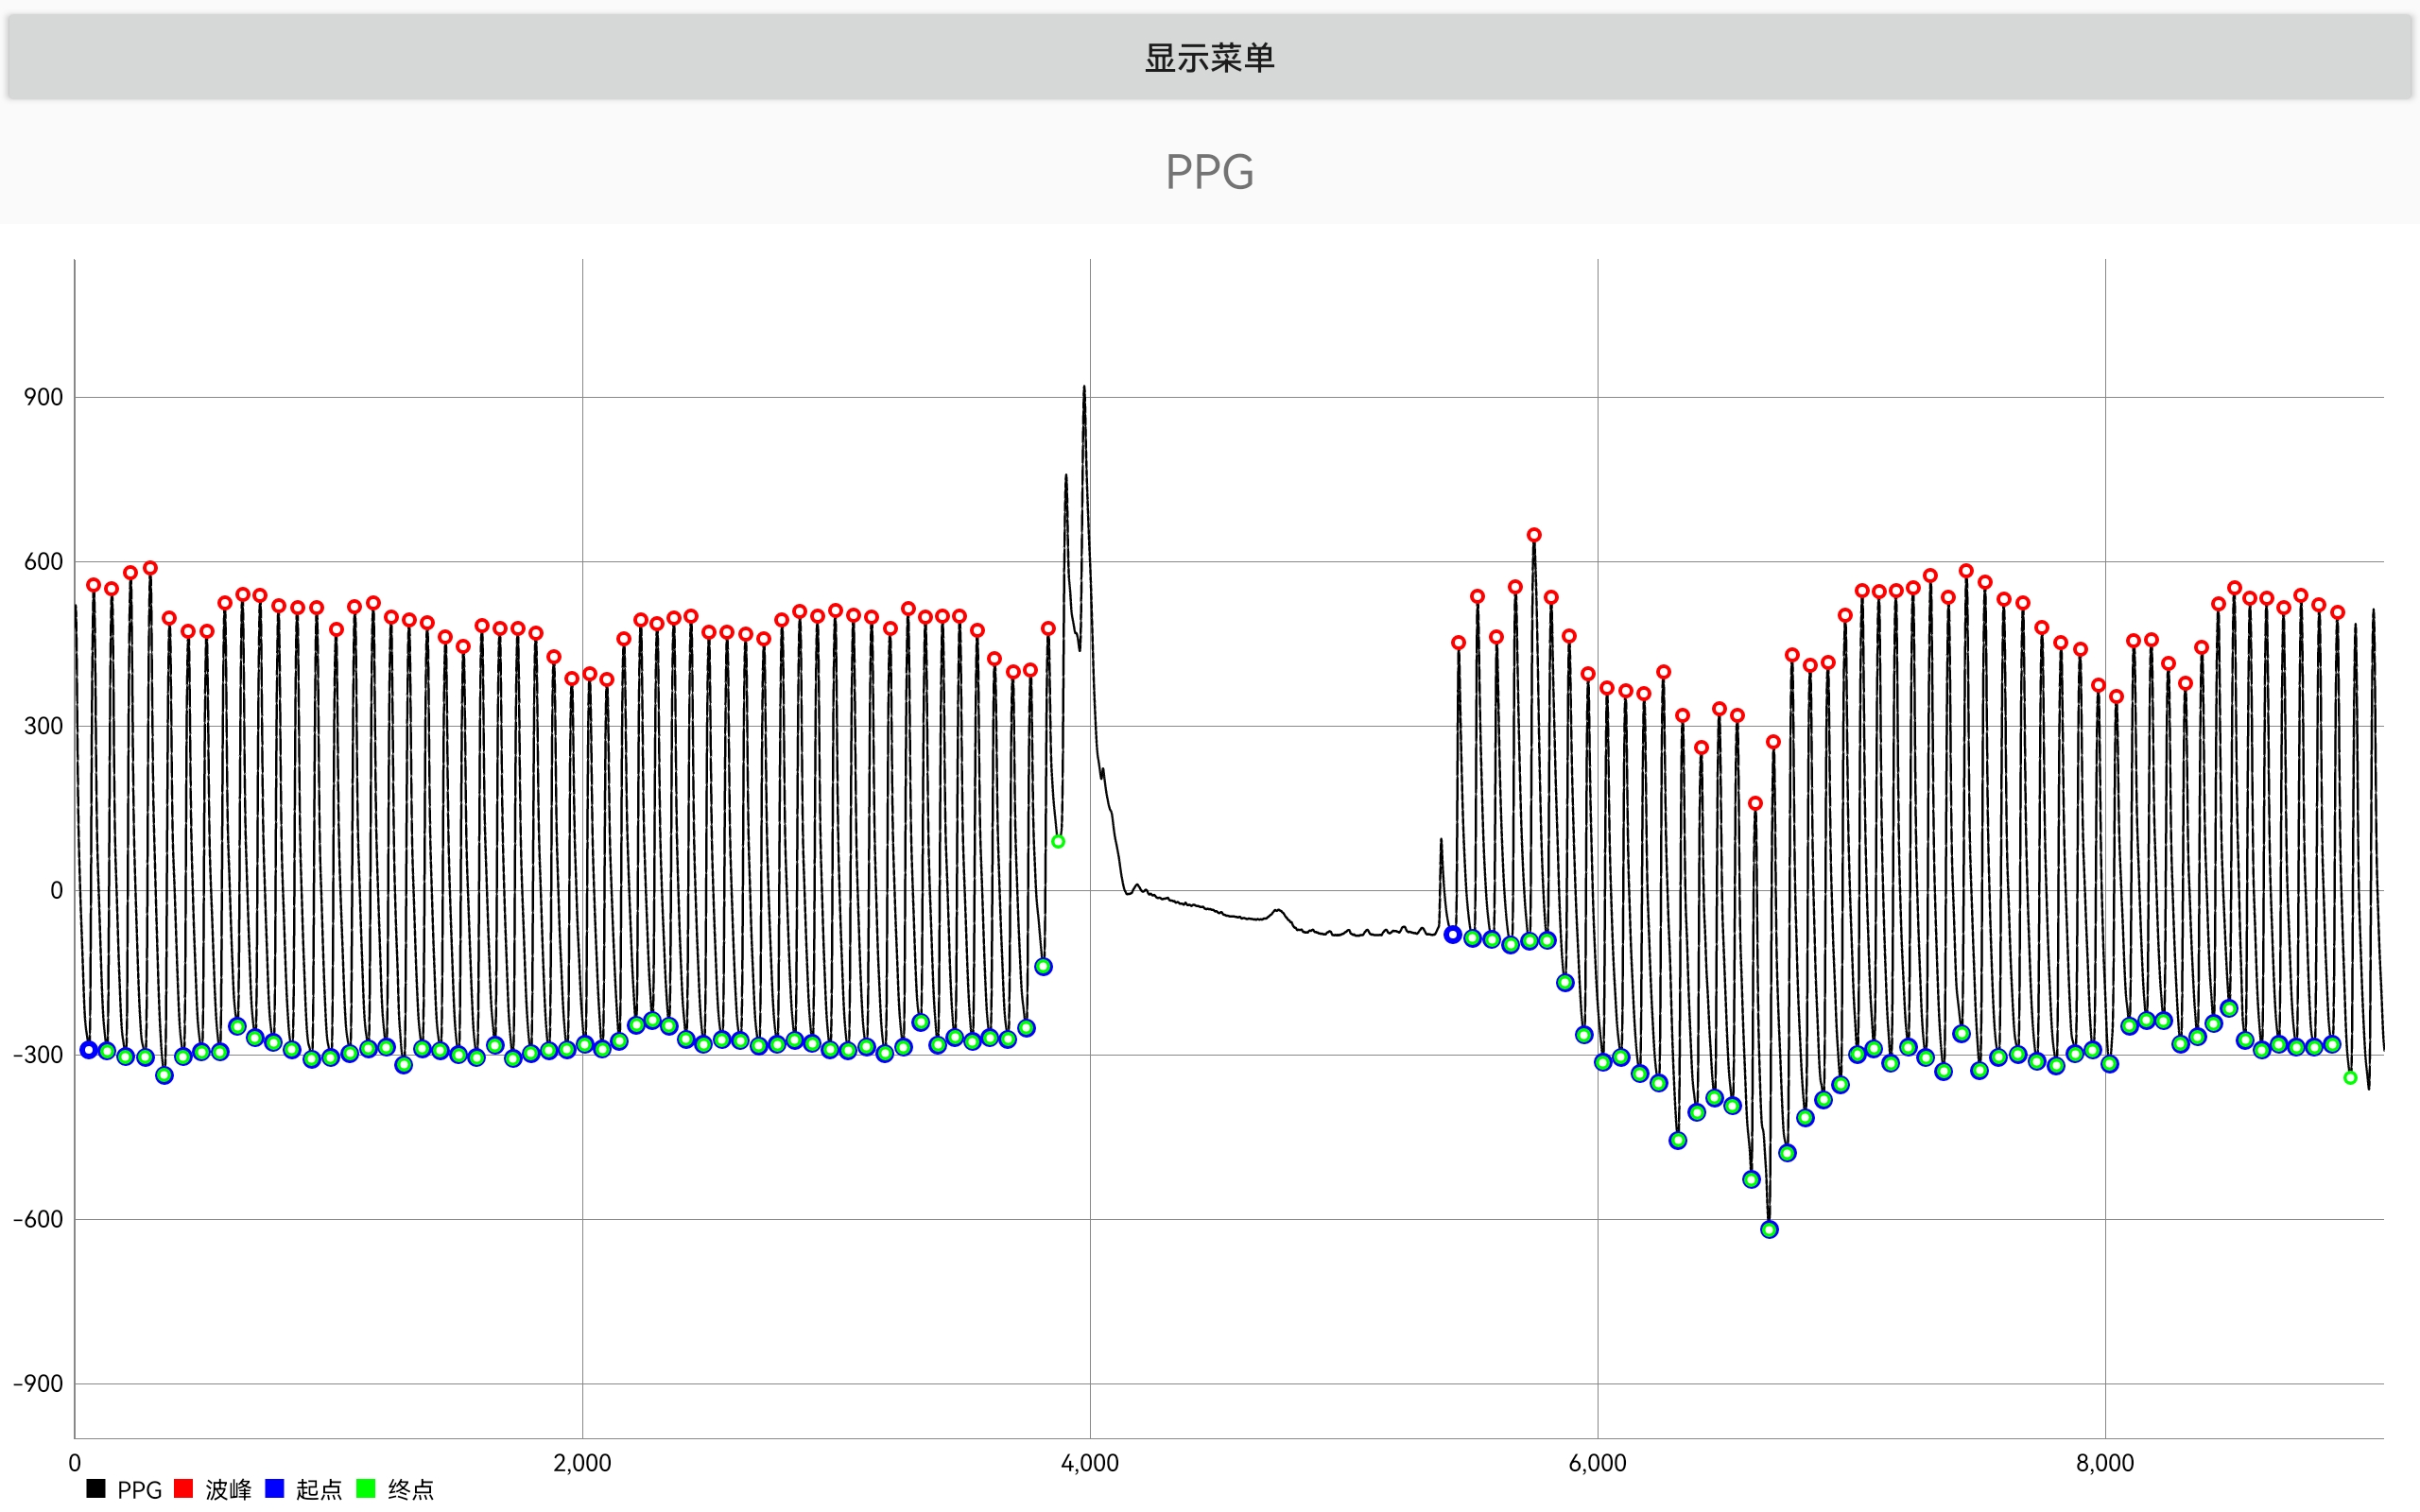
\includegraphics[width=0.9\linewidth]{software/android_demo}
    \caption{\label{fig:android_demo}Android客户端对被试dmq的PPG数据检测结果图}
\end{figure}
\begin{figure}[htbp]
    \centering
    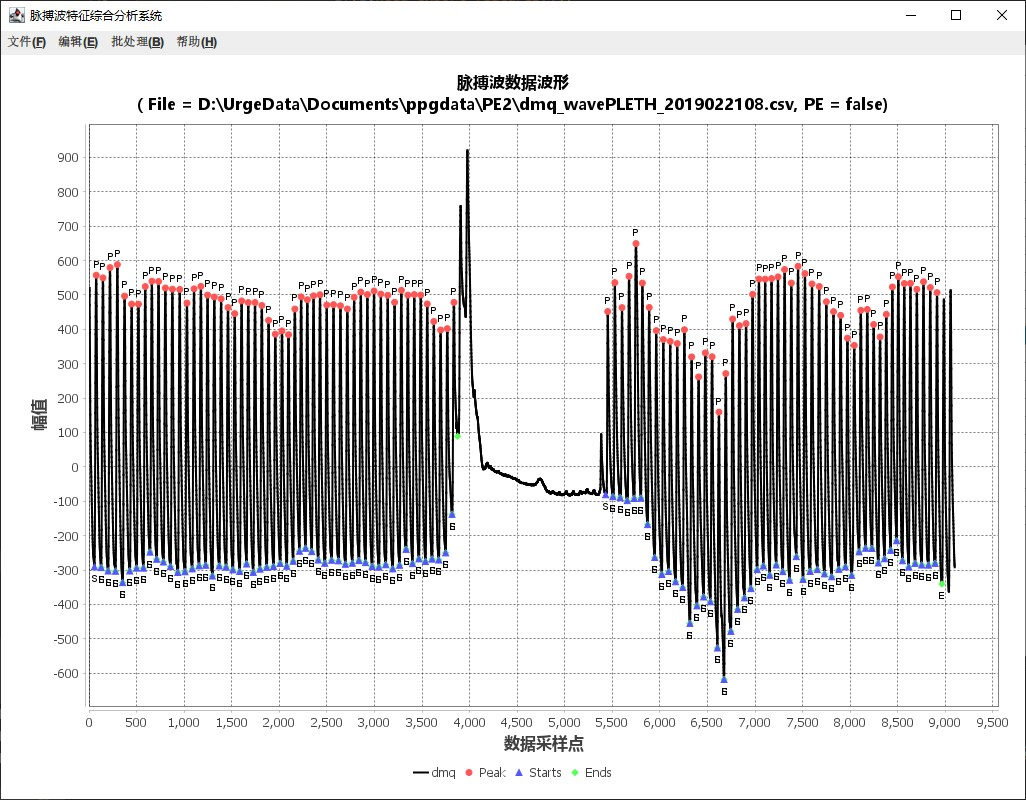
\includegraphics[width=0.9\linewidth]{software/pc_demo}
    \caption{\label{fig:pc_demo}PC客户端对被试dmq的PPG数据检测结果图}
\end{figure}

为测试验证两个平台下的客户端软件,分别两者处理相同的PPG数据,结果表明,两个平台下的检波效果完全一致,如\autoref{fig:android_demo}与\autoref{fig:pc_demo}所示。
而进一步比较两个平台下的文件输出结果,得到的处理结果也相同。这表明软件系统的多平台客户端程序的处理结果具有一致性。

关于客户端网络通讯功能的测试与验证可参见下一小节。

\subsection{云服务器端程序的测试与验证}
云服务器端程序的测试主要包括两方面,首先为不同客户端软件与云服务器的网络连接测试;其次为不同客户端软件与云服务器的整体功能性测试,即接收数据并调用模型进行识别预测的
完整功能性测试。

一、测试环境与设备

云服务器模块在设计时是可以直接使用第三方商业公司提供的具有公网IP地址的服务器进行真正的云部署。但出于方便开发的角度,在本软件系统的研发过程中,暂时仅使用了
局域网进行环境搭建模拟与后续测试。在此条件下,软件系统的整体物理设备组成架构如\autoref{fig:system_net}所示。

在\autoref{fig:system_net}中,笔记本A作为局域网内的主机服务器,运行着软件系统的云服务器端程序;笔记本B与平板电脑分别作为PC客户端与Android端的运行平台;
而这些设备通过路由器搭建的无线局域网联络在一起。这些设备的具体生产厂商及型号、运行操作系统等硬件信息如\autoref{tab:system_devices}所示。
\begin{figure}[htbp]
    \centering
    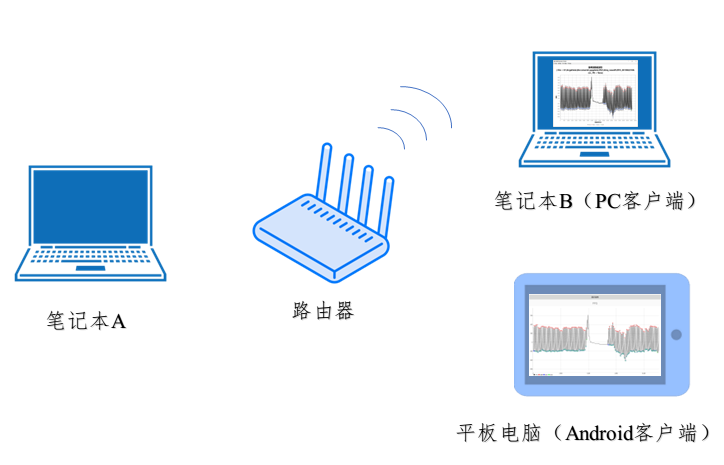
\includegraphics[width=.6\linewidth]{software/system}
    \caption{\label{fig:system_net}软件系统在局域网下的部署示意图}
\end{figure}

\begin{longtblr}
    [
        theme                   = {zju},
        caption                 = {软件系统所使用的各网络设备型号},
        label                   = {tab:system_devices},
    ]
    {
        width                   = 0.8\linewidth,
        colspec                 = {X[1,c,m]X[1,c,m]X[2,c,m]X[1,c,m]},
        hline{1,Z}              = {\thickline},
        hline{2}                = {\thinline},
        rowhead                 = 1,
        row{1}                  = {font=\headfont},
        row{2-Z}                = {font=\nonheadfont},
    }
    设备代号&制造厂商&型号&系统版本\\
    笔记本A&中国小米&Redmibook 15 Pro&Win 10\\
    笔记本B&中国小米&Redmibook 15 Pro&Win 11\\
    路由器&中国华为&WS5102&\\
    平板电脑&中国小米&Redmi Pad SE&Android 12\\
\end{longtblr}

二、网络连接的测试与验证

如\autoref{tab:post_paras}所示,当客户端通过POST方法与云服务器端进行通讯时,传递的参数信息中包含了此次由客户端程序发起通讯的时间。
因此,云服务器只需要记录下接收到数据信息的时间即可验证此次网络通讯连接成功,同时也可以利用这两个时间的间隔评估网络延迟等信息。需要注意,
在测试网络延迟前,各网络设备均需提前与标准网络时间服务器进行过校正对齐。

按上述步骤,即可得到本论文采集得到的79名被试数据经客户端与云服务器端的网络连接延时后,并可进一步得到所有数据文件平均延时,其结果如\autoref{tab:time_delay}所示。
可以看到,上述数据经由PC客户端与Android客户端与云服务器均能进行有效通讯,没有出现数据丢失等现象,同时
具有较小的网络延迟。这可能与测试环境在局域网内搭建、测试数据整体传输量较小等因素有关。

\begin{longtblr}
    [
        theme                   = {zju},
        caption                 = {不同客户端上传文件的平均网络连接延迟对比},
        label                   = {tab:time_delay},
    ]
    {
        width                   = 0.6\linewidth,
        colspec                 = {X[1,c,m]X[1,c,m]},
        hline{1,Z}              = {\thickline},
        hline{2}                = {\thinline},
        rowhead                 = 1,
        row{1}                  = {font=\headfont},
        row{2-Z}                = {font=\nonheadfont},
    }
    客户端平台&平均延时(ms)\\
    PC&0.594\\
    Android&0.517\\
\end{longtblr}

三、预测模型的测试与验证

在客户端软件中选择打开原始PPG数据文件后,当客户端完成了预处理后,处理结果会被上传至云服务器端。
云服务器端调用PE识别模型并返回结果,不同平台下的返回结果如\autoref{fig:pc_response}与\autoref{fig:android_response}所示。

\autoref{fig:pc_response}与\autoref{fig:android_response}分别对应着被试cmf的原始数据在PC客户端与Android客户端的
\begin{figure}[htbp]
    \centering
    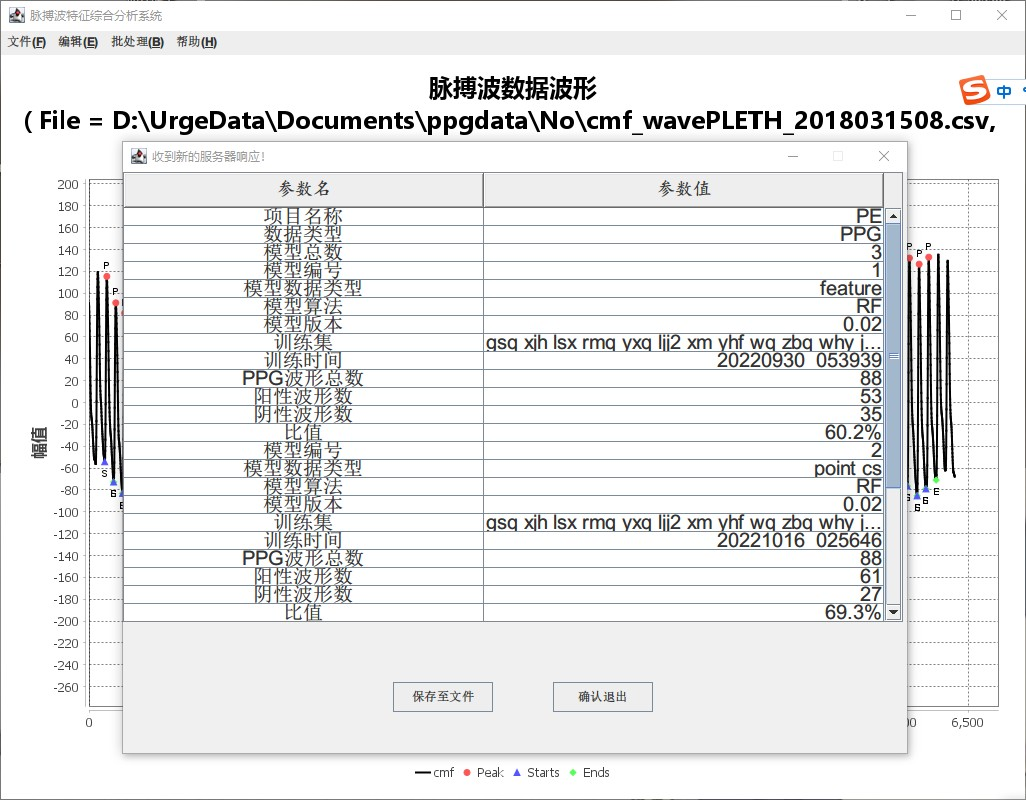
\includegraphics[width=.9\linewidth]{software/pc_response}
    \caption{\label{fig:pc_response}PC客户端接收到的请求响应示意图}
\end{figure}
\begin{figure}[htbp]
    \centering
    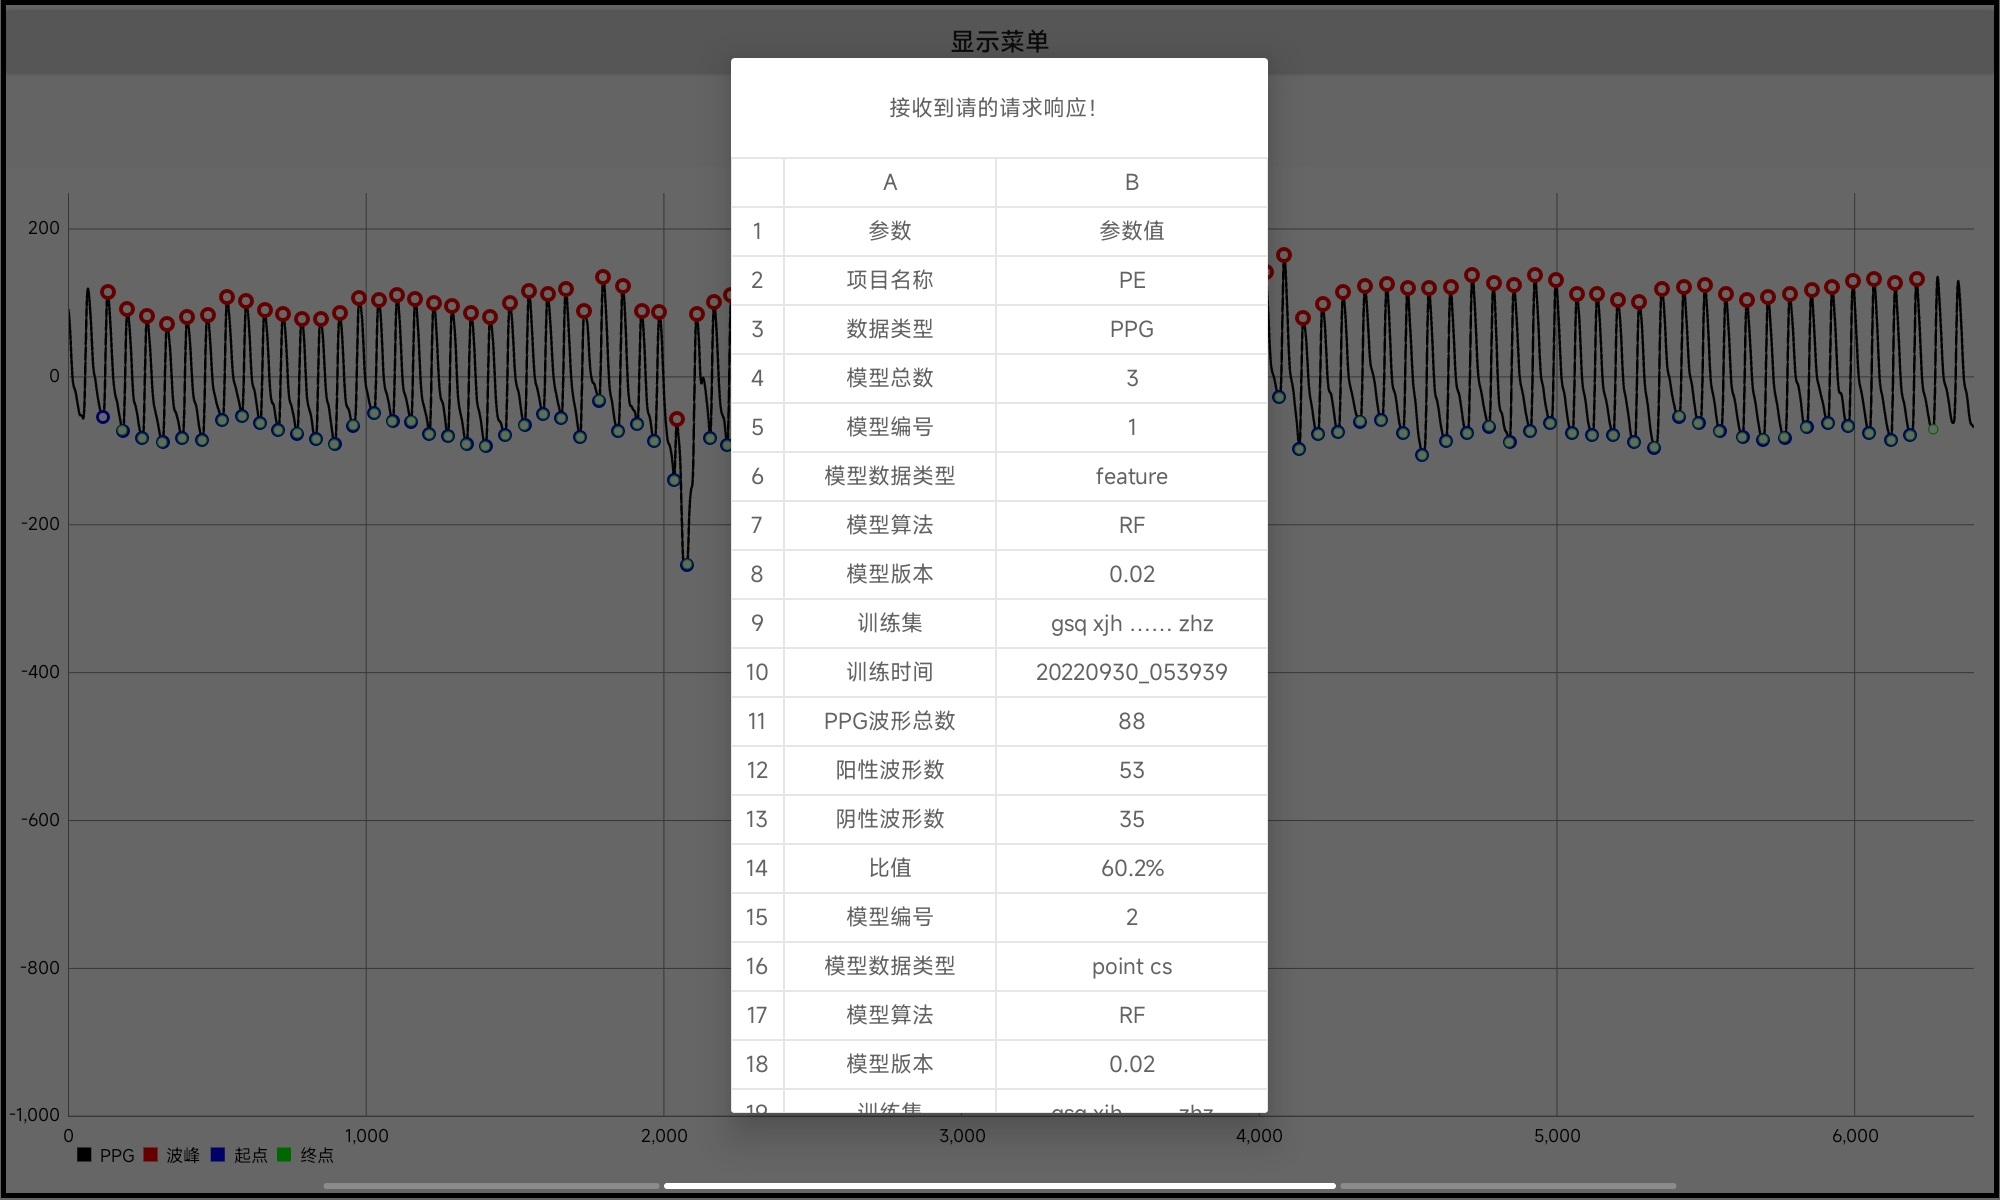
\includegraphics[width=.9\linewidth]{software/android_response}
    \caption{\label{fig:android_response}Android客户端接收到的请求响应示意图}
\end{figure}
\noindent
响应结果,而
被试cmf数据的数据结果分别对应着\autoref{tab:model_detail}与\autoref{tab:model_detail2}的相关内容。
云服务端的响应结果分别在\autoref{fig:pc_response}与\autoref{fig:android_response}以表格的形式进行了呈现。%相关参数的意义可参考\autoref{tab:json_response}。
特别地,由于对于基于被试的研究而言,PPG的分析数据包括时域特征与原始采样值两大类;
而对于原始采样值而言,又使用了两种PPG波形的对齐策略。因此,\autoref{fig:pc_response}与\autoref{fig:android_response}中的模型总数的这一参数值均为3。

\subsection{数据库的测试与验证}
由于软件系统使用了MySQL数据库作为后台,因此,当软件系统正常运后,可直接在命令行下连接至数据库,查询数据库的存储状态。
在命令行下模式下,键入命令$mysql\ -u\ root\ -p$后,输入数据库密码,即可登陆数据库;随后使用SQL语言$use\ bme207$即可选中软件系统在MySQL软件中使用的数据库;
最后,使用SQL语言$show\ Tables$即可查询数据库bme207下所有数据表的状态,得到的结果如\autoref{fig:mysql_db}所示。
\begin{figure}[htbp]
    \centering
    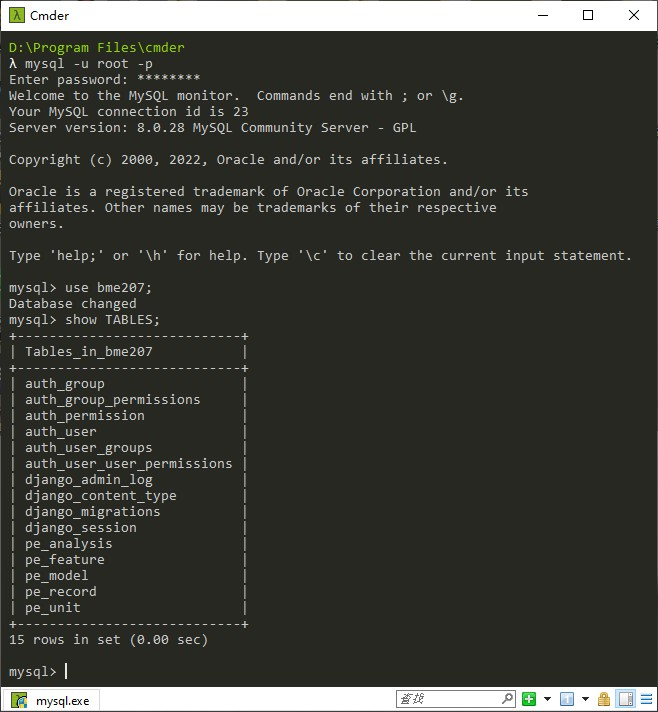
\includegraphics[width=0.55\linewidth]{software/mysql}
    \caption{\label{fig:mysql_db}命令行下查询MySQL数据库结构示意图}
\end{figure}

如\autoref{fig:mysql_db}红色框选部分所示,上节中介绍的5张自定义数据表均已按预期生成。与此同时,\autoref{fig:mysql_db}也存在着Django框架自动生成的一些数据表。而这些数据表的详细
作用如\autoref{tab:django_db}所示。
\begin{longtblr}
    [
        theme                   = {zju},
        caption                 = {Django框架自动生成的数据表及其作用},
        label                   = {tab:django_db},
    ]
    {
        width                   = \linewidth,
        colspec                 = {X[1,c,m]X[3,c,m]},
        hline{1,Z}              = {\thickline},
        hline{2}                = {\thinline},
        rowhead                 = 1,
        row{1}                  = {font=\headfont},
        row{2-Z}                = {font=\nonheadfont},
    }
    数据表名称&作用\\
    auth\_group&该表维护用户组信息\\
    auth\_group\_permissions&该表维护了用户权限和用户组别之间的多对多关系\\
    auth\_permission&该表维护了用户权限信息\\
    auth\_user&该表维护了用户信息\\
    auth\_user\_groups&该表维护了用户组信息与用户信息之间的多对多关系\\
    auth\_user\_user\_permissions&该表维护了用户权限信息和用户信息之间多对多关系\\
    django\_admin\_log&该表记录了用户在admin页面的操作日志\\
    django\_content\_type&该表记录了项目中所有app与model之间的对应关系\\
    django\_migrations&该表维护了Django项目所有的数据迁移记录信息\\
    django\_session&该表维护了所有session信息\\
\end{longtblr}

\begin{figure}[htbp]
    \centering
    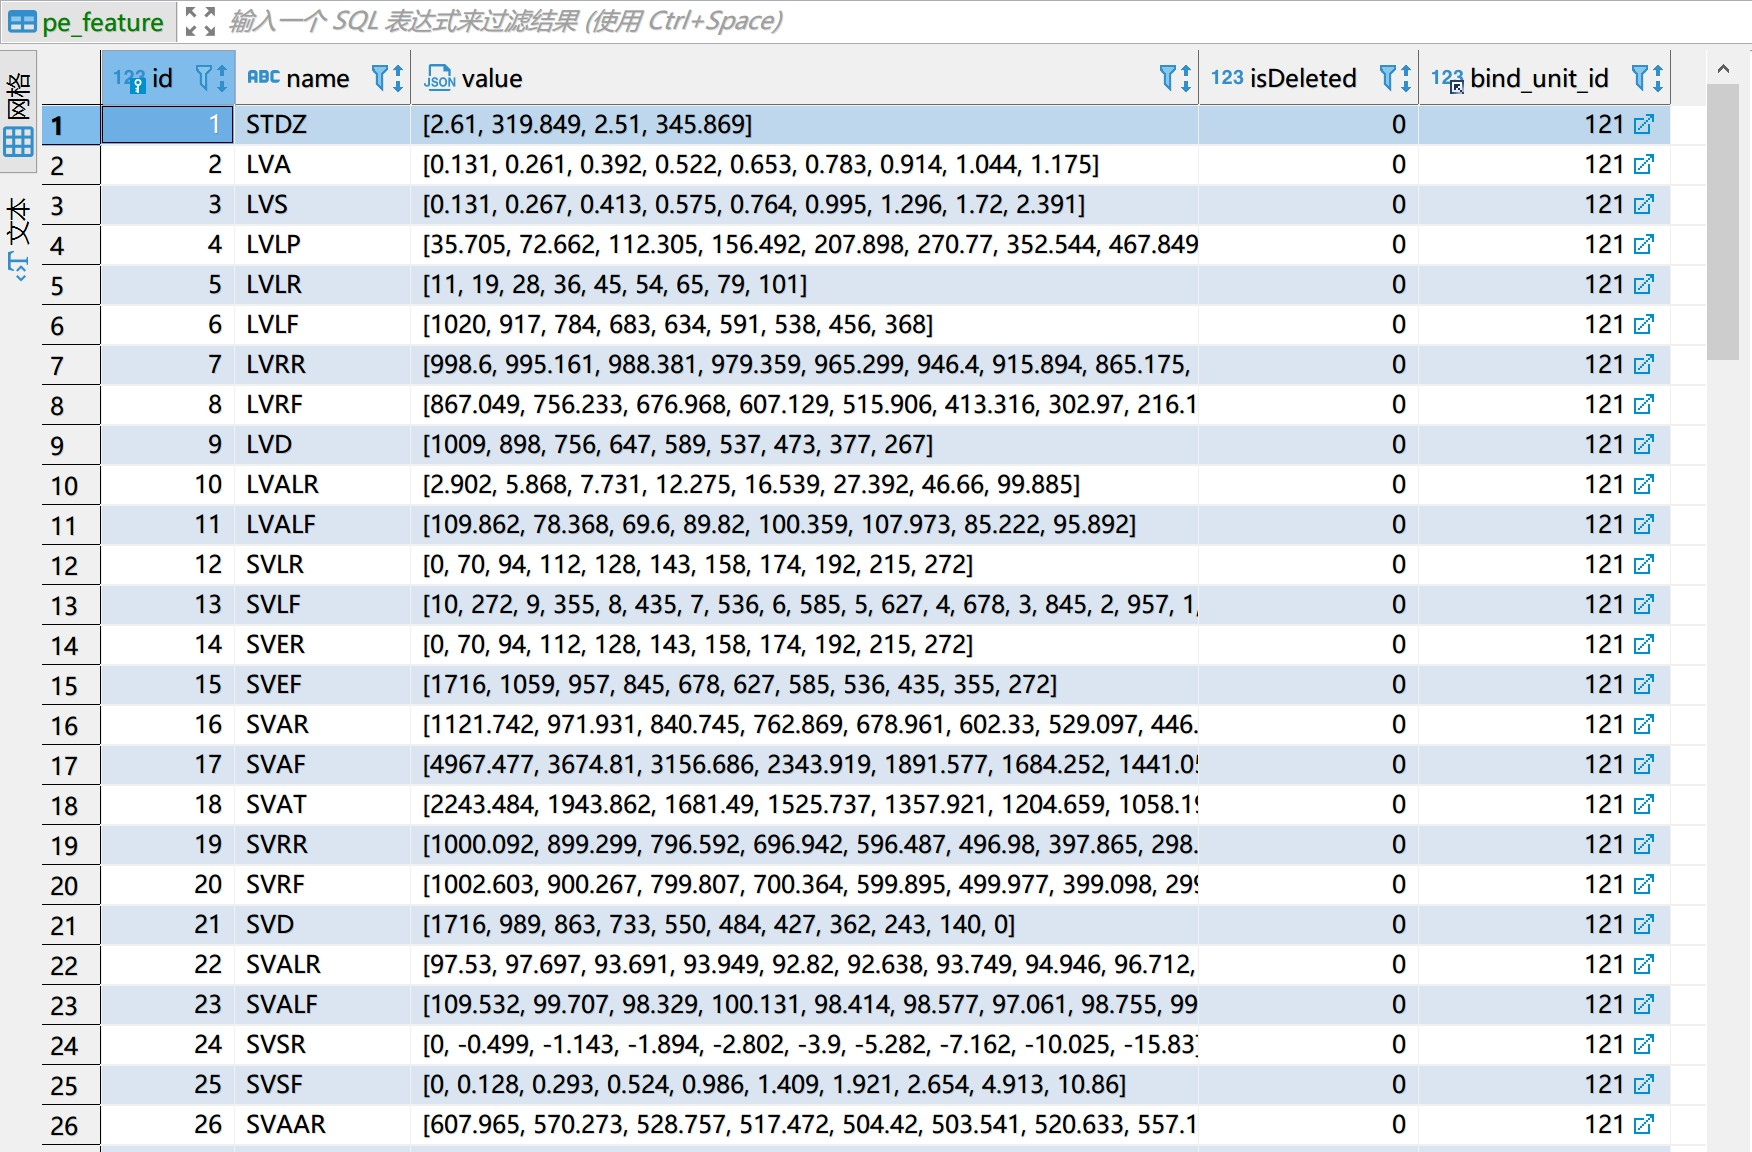
\includegraphics[width=0.9\linewidth]{software/feature_db}
    \caption[Feature数据表的存储情况示意图]{\label{fig:feature_db}Feature数据表的存储情况示意图}
\end{figure}

在\autoref{fig:mysql_db}的查询结果的基础上,借助开源图形界面化的数据库管理软件DBeaver可以进一步地直接观察各数据表的存储状态\cite{dbeaver}。
查询\autoref{fig:mysql_db}的Feature数据表结果如\autoref{fig:feature_db}所示,可以看到该数据表已按\autoref{tab:data_table_feature}的设计进行了
多种PPG特征数据的有效存储。

\section{小结}
本章基于PPG信号的设计并实现了一款具有较强的兼容性与拓展性的PE识别分析软件系统,该软件系统具有完整可用的基于PPG信号的PE识别分析功能。
首先,详细分析了软件系统的研发需求。其次,介绍了软件系统的整体性多模块化设计。随后,针对各个模块的设计需求,
对各模块的实现工作进行了介绍。对各模块进行的测试结果表明,软件系统的各项功能均能按照设计预期正常工作,具有良好的检测准确性与可靠性。